
%=============================================
\chapter{A Testbed Environment for Task Development }\label{c1}
%\textbf{~20 pages}

%\textbf{Currently contains \the\numexpr\getpagerefnumber{c2}-\getpagerefnumber{c1}\relax  pages | Calculated dynamically.}

\section{Introduction}


% \subsection{Service Robotics}
% % \textbf{~0.5 pages}

% %We may think that robots were invented to serve humans.
% % Phrase trop général et subjectif ! Ce n'est pas scientifique

% %Consequently, what is the disparity between the terms service robots and service robotics? 
% % Ne pose pas de tel questions mais pose des definition

% %Although this is a valid point, to distinguish from the initial wide usage of robots in manufacturing, the term service robotics was invented to show robotics technologies and applications in nonmanufacturing areas. 
% % Valid point, ca veut dire que tu le prouves ! Ce n est pas le cas !! Prefere poser des definitions plutot que des discussions


% The term service robots was intended to highlight emerging markets for the new types of robots. It was coined to distinguish from the initial wide usage of robots in manufacturing, as robotics technologies and applications were extended to nonmanufacturing areas. This was the motivation behind initiating the Service Robots Technical Committee (TC) within the IEEE Robotics and Automation Society (RAS) in 1995. 
% OK pour ce paragraphe

% \subsection{ UAV Functionality Development}
% %\textbf{~0.5 pages}
% %[Brief overview of UAV Research.] 

% Presently UAVs are beginning to be major inroads into geographical mapping, site inspection, agriculture, and search and rescue \cite{kovacs_hildmann_2019}.

% % What are the limits ??? What ? Why ? How ?
% % [Why a UAV Platform??]
% However, there remains large challenges to implementation of UAVs: the reliability of software, the limits on the hardware, test and validation of new elements on pre-existing systems \cite{larrabee_chao_kumar_gururajan_gu_napolitano_2013}. These machines are ideally tested in close-to-real conditions. In this way, flight performance monitoring systems are a fundamental asset to further development in this field.

% %\color{ForestGreen} [How we choose to proceed.] \color{black} 
% In order to stay relevant to this evolving field, a development setup has been put in place. It may be used for testing new technologies and for deploying robotic systems.

% \subsection{ Offboard Compute}
% %\textbf{~0.5 pages}
% %[Brief overview of GCS.] 
% Computation  offloading  is  emerging  as a  new  trend,  enabling  robots  with  more 
% powerful  computation resources.  It  helps  them  to  overcome  the  \textbf{hardware  and  software limitations}  by  leveraging parallel  computing  capabilities  and the  availability  of  large  amounts  of  resources  on a separate system, either in the cloud, or on a local computation system.

% Empowering robots with cloud computing comes with a fundamental tradeoff. Offloading the execution of a computationally intensive algorithm to the cloud can \textbf{reduce resource
% utilization}, including CPU, memory, and the battery. However, this comes with a cost: communicating with cloud resources over a congested network increases latency and can lead to delay for real-time applications.

% GCS hardware refers to the complete set of ground-based hardware systems used to control the UAV. This typically includes the Human-Machine Interface, computer, telemetry, video capture card and aerials for the control, video and data links to the UAV. 

% What are the limits ??? What ? Why ? How ?
% [Why a GCS??]

% [How we choose to proceed.] 

%\subsection{Context}

% The term service robots was intended to highlight emerging markets for the new types of robots. It was coined to distinguish from the initial wide usage of robots in manufacturing, as robotics technologies and applications were extended to nonmanufacturing areas. This was the motivation behind initiating the Service Robots Technical Committee (TC) within the IEEE Robotics and Automation Society (RAS) in 1995. 

% swarm_engineering_field}
According to \citetitle{swarm_review} \cite{swarm_review}, swarm robotics is an approach to collective robotics that takes inspiration from the self-organized behaviors of social animals. Through simple rules and local interactions, swarm robotics aims for robust, scalable and flexible collective behaviors for the coordination of large numbers of robots. In contrast, the term swarm engineering \cite{swarm_engineering} describes the design of predictable, controllable robot swarms with well-defined goals and the ability to function under certain conditions. Swarm engineering focuses mainly on concepts that could be relevant for real-world applications, therefore shifting swarm robotics to engineering applications. 
% multi_robot_why}
We motivate a smarter ecosystem for task development upon drones by beginning with the infrastructure for new technologies and for prototyping functionalities. A centralised swarm framework serves to set up flight performance monitoring systems, a fundamental asset to the development of robots and multi-robot groups \cite{gcs_validation}.

Multi-robot systems and swarms of unmanned aerial vehicles (UAVs) in particular have many practical applications.  \citetitle{overview_uavsensors} \cite{overview_uavsensors} from March 2021 shows applications as diverse as surveillance and monitoring, inventory management, search and rescue, or in the entertainment industry. Swarm intelligence has, by definition, a distributed nature. Yet performing experiments in truly distributed systems is not always possible, as much of the underlying ecosystem employed requires some sort of central control. Indeed, in experimental proofs of concept, most research relies on more traditional connectivity solutions and centralized approaches \cite{gcs_validation}\cite{buzz_swarm_stack}.

%\subsection{Motivation}

In recent years there have been significant advancements in this research field. However, very rarely do UAV swarms leave the controlled and safe environment of laboratories, and when they do it is for short-duration experiments. The current use of swarms is generally based on custom, centralized solutions, in environments with reliable communication \cite{buzz_swarm_stack}. There remains large challenges to reliable flight of UAVs: the reliability of software, the limits on the hardware, test and validation of new elements on pre-existing systems \cite{gcs_validation}. A further challenge concerns multi-robot functionality. Current UAVs have very limited functionality for multi-robot coordination. Market drones are too limited for swarm research, as they only supports a single point-to-point link between a program and the drone, thus, a program can only communicate with a single drone. 

% c1_thesisgoal}
In line with the thesis goal, we seek to better understand how distributed systems can offer smart assistance to multi-robot development. We explore research and techniques designed to coordinate multiple robots.



\pagebreak
\section{Related Work}
%\textbf{~4 pages}

In this section, we examine how researchers tackle the challenge of swarm engineering in the past. Prior work exists in a variety of drone laboratories \cite{flightmare} \cite{fma_paper}. Drones Spatial Localization, UAV Architectures and UAV Swarm Frameworks require tradeoffs.

\subsection{UAV Spatial Localization}
%\textbf{~1 pages}
%\textbf{ Discussing different Localization Technologies in Comparison. }

\begin{marginfigure}%
  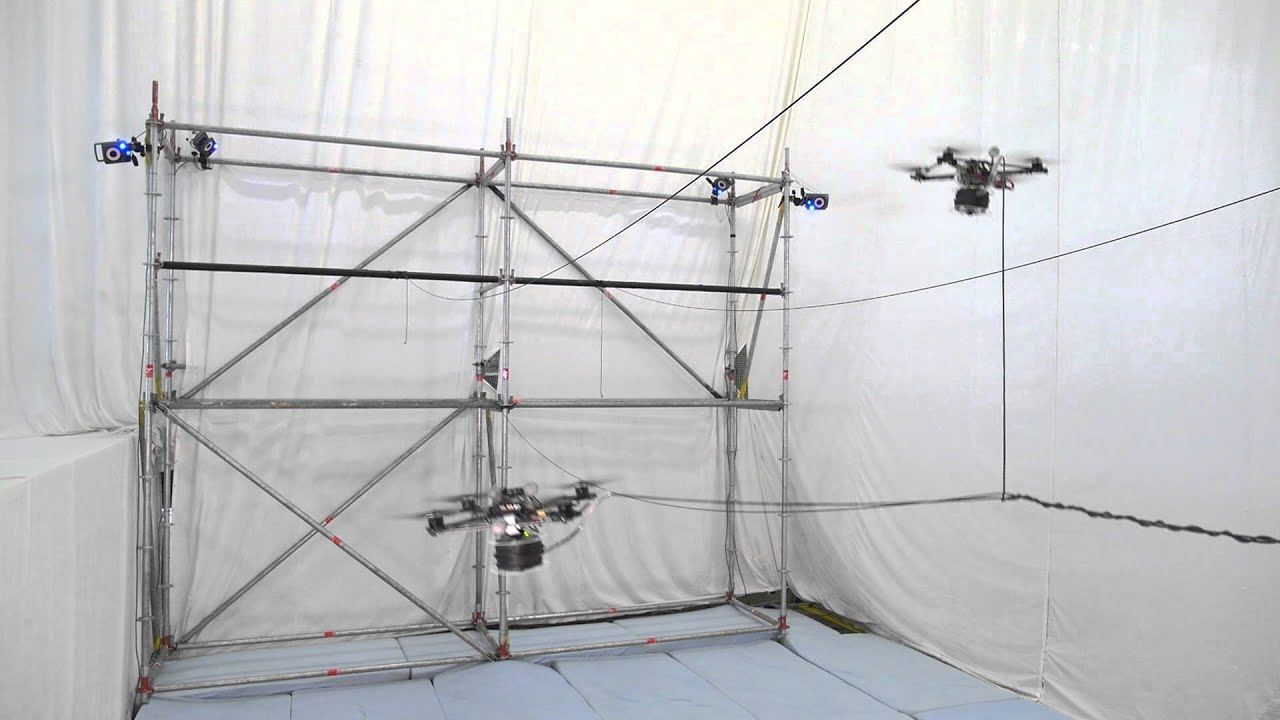
\includegraphics[width=\linewidth]{images/drones_setup.jpg}
  \caption{An example of drones tracked by two motion capture cameras.  }
  %\label{fig:marginfig}
\end{marginfigure}

The Flight of UAVs, as with any robotic system, requires accurate positioning. However, a drone suffers from cumulative drift in position data \cite{uav_components}. In order to achieve autonomous flight, a drone will need to know if it is following a trajectory correctly. A localization technology allows for this
centimeter level accuracy.

It is by using highly precise equipment, that UAVs can have highly precise state estimation. This setup includes the selection of onboard positioning systems as well as external positioning solutions. We focus on optical motion capture coupled with algorithms for state estimation primarily a set of technologies commonly used by UAV laboratories\cite{phan_hönig_ayanian_2018} \cite{laclau_tempez_ruffier_natalizio_mouret_2020} \cite{fma_paper}:. 

The high level of precision from a motion capture system allows us to synchronously hover multiple UAVs. The tracker precision can reach sub-millimeter accuracy, and drones are hovered at a precision of a few centimeters.

%     \item What are the trade-offs of the different alternatives and why did you choose a particular one -->> MOTION CAPTURE...
%     \item How does your contribution relate to prior work

% [Other setups can be listed here.] 


\subsection{UAV Architectures}
%\textbf{Discussing several UAV Architectures in Comparison }

UAVs such as AscTec Pelican, Parrot AR.Drone, and Erle-Copter are other examples of UAVs commonly used in the literature. These MAVs have Software Development Kits (SDK) that enable applications from third-party developers to communicate with the drones. However, both SDKs are too limited for swarm research, as they only supports a single point-to-point link between a program and the drone, thus, a program can only communicate with a single drone.

\begin{marginfigure}%
  \includegraphics[width=\linewidth]{images/DSCF0871.jpg}
  \caption{The Crazyflie 2.1 miniature quadcopter.  }
  %\label{fig:marginfig}
\end{marginfigure}

In comparison, the Crazyflie packages the full robotic stack. This robotic stack includes its own state estimator, control architecture and trajectory follower, which work out of the box. FreeRTOS handles the scheduling of processes and control the flight calculations. The Crazyflie contains a 32-bit, 168MHz ARM microcontroller with floating-point unit that is capable of significant onboard computation. The FreeRTOS firmware is opensource and modifiable. 

 The Crazyflie’s small size makes it suitable for indoor flight in dense formations. As a result, it has been used widely in research. As of 2021, this drone is used to validate research: from new algorithms for agile flight \cite{laclau_tempez_ruffier_natalizio_mouret_2020} to drone swarm research \cite{phan_hönig_ayanian_2018}.





 
\subsection{UAV Swarm Frameworks}
%\textbf{~1 page: }
%\textbf{An Overview of Swarm Frameworks }

Unmanned Aerial Vehicle (UAV) swarms have been used indoors for formation flight and collaborative behaviors, outdoors to demonstrate swarming algorithms, and in the media for artistic shows. According to \textit{\citename{swarm_review}{author}} \cite{swarm_review}, The group of robots has some special characteristics, which are found in swarms of insects, that is, decentralised control, lack of synchronisation, simple and (quasi) identical members. In this section, we explore the requirements placed on the software framework for interacting with a robot swarm. 

% [Challenges.] \cite{phan_hönig_ayanian_2018}.

\cite{pinciroli_lee-brown_beltrame_2015} \hspace*{0.3cm} \textit{\citename{pinciroli_lee-brown_beltrame_2015}{author}}
\hspace*{0.5cm} discuss the key requirements a successful programming language for swarm robotics must meet. According to them, the level of abstraction need be adapted to the task at hand. The complexity of concentrating on individual robots and their interactions, i.e., a bottom-up approach, increases steeply with the size of the swarm. Conversely, a purely top-down approach, i.e., focused on the behaviour of the swarm as a whole, might lack expressive power to fine-tune specific robot behaviors. The runtime platform of the language must ensure acceptable levels of \textbf{scalability} (for increasing swarm sizes) and \textbf{robustness} (in case of temporary communication issues). 

\cite{fma_paper} \textit{\citename{fma_paper}{author}}
\hspace*{1cm} present The Flying Machine Arena. This was put in place in 2014 with the goal of becoming a "demo-and-development" arena. They include both single and multi-robot experiments. One key element of their work is that the UAV swarm can be heterogeneous. Additionally, the position controller runs offboard, that is, the UAVs all rely on a companion computer to position themselves. The additional computational power is used for a latency compensation algorithm to improve accuracy for high-speed flights. Despite this, the framework remains robust: swarms of up to 5 UAVs are flown on a regular basis.

\cite{phan_hönig_ayanian_2018} \textit{\citename{phan_hönig_ayanian_2018}{author}}
\hspace*{1cm} define a system architecture for a large swarm of miniature quadcopters flying in dense formation indoors. 
%[why] 
The main challenges in swarm robotics are addressed in this framework, namely by reducing communication latency to 26ms.
%[how] 
This is done in major part via the structure of messages broadcasted to the UAV. Preiss et al. \cite{phan_hönig_ayanian_2018} use a programmable UAV with an onboard position controller, making the system more robust to communication packet drops. With this method, a swarm of 49 Crazyflies have been flown using 3 radios. 
% [Conclusion.]
As a result, the drone swarm framework allows for robotics developers to send commands to drones in a fleet. A scalable and robust run-time platform is, in this way, a key element for real-world deployment of swarm behaviors.

\subsection{UAV Software and Middleware}

%\textbf{~1 page } 
%\textbf{ Middleware approaches in comparison }

% Computation  offloading  is  emerging  as a  new  trend,  enabling  robots  with  more 
% powerful  computation resources.  It  helps  them  to  overcome  the  hardware  and  software limitations  by  leveraging parallel  computing  capabilities  and the  availability  of  large  amounts  of  resources  in  the  cloud. The \textbf{performance  gain}  of  computation  offloading  in cloud  robotics  is  still  an  ongoing  research  problem  because of  the conflicting factors that affect the performance. 

% There are a few operating systems or robot middleware worth mentioning:
% \begin{itemize}
%     \item \textbf{Microsoft Robotics Developer Studio}: a multiplatform system, created by Microsoft. It is free and provides a simulation tool; however, it is only compatible with Windows and is programmed with a managed .NET language (preferably C\#).

%     \item \textbf{NAOQi}: open source robotics system produced for the NAO robot by Aldebaran Robotics, and programmed in C++ or Python.

%     \item \textbf{URBI} : produced by the French company Gostai. URBI is a good multi-platform, open source and offers its own scripting language (URBIScript), although it is also programmed in C++.
% \end{itemize}

UAVs have a long tradition of being controlled with the Robotic Operating System. ROS is a meta-operating system designed for the construction of distributed systems. It provides a set of extensible tools for managing distributed robotic applications.
The main goals of ROS are package management, hardware abstraction, low-level device control, message exchange between processes, and implementation of several functionalities. As a result, there are many ROS packages devoted to controlling such UAVs as individuals. 

However, using multiple UAVs creates entirely new challenges that such packages cannot address. These new challenges include, but are not limited to, the physical space required to operate the robots, the interference of sensors and network communication, and safety requirements. In \cite{hönig_ayanian_2020} and \cite{phan_hönig_ayanian_2018}, \citename{phan_hönig_ayanian_2018}{author} thus motivates the use of a hardware abstraction layer on top of the Crazyflie. This abstraction layer, in the form of a ROS layer, is only used on the PC controlling one or more Crazyflies. The ROS driver sends the data to the different quadcopters using the protocol defined in the Crazyflie firmware.

\cite{hönig_ayanian_2020} \hspace*{0.3cm} \textit{\citename{hönig_ayanian_2020}{author}} \hspace*{0.5cm} 
demonstrates interoperability between the PC and UAV components.  The \textit{crazyflie\_ros} framework helps wrap CRTP within a ROS framework, which is useful for scenarios of hovering and waypoint following from a single robot to the more complex multi-UAV case. It provides not only standard operating system services (hardware abstraction, contention management, process management), but also high-level functionalities (asynchronous and synchronous calls, centralised database, a robot configuration system, etc.). Additionally, this includes command-line tools and a GUI for mass rebooting, firmware updates, firmware version query, and battery voltage checks over the radio.

\begin{marginfigure}%
  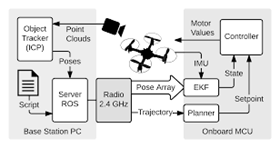
\includegraphics[width=6cm, center]{images/testbed/controlloop_bw.png}
  \caption{Overview of the Crazyswarm Control Loop, as per the Crazyswarm official documentation (August 2021) \cite{crazyswarm_docs}}
  %\label{fig:marginfig}
\end{marginfigure}

\cite{preiss_hönig_sukhatme_ayanian_2017} \hspace*{0.3cm} \textit{\citename{preiss_hönig_sukhatme_ayanian_2017}{author}}
\hspace*{0.5cm} furthers this work by offering all the necessary components for controlling multiple drones remotely, by relating the drone flight controller of the Crazyflie to a set of controllers on the PC, but also by offering ways to send trajectories to the drones in realtime.  Crazyswarm attempts to couple an external motion capture technology like Optitrack with the rest of a drone’s control loop: knowing its position, the drone will be able to generate and follow a trajectory more precisely. When viewing a single body, motion capture certainly has sub-millimeter accuracy. However, as the number of drones increases, there are two limiting factors to the reliability of the control loop: the first is recognition of the drones by the optical capture system, and the second is low communication bandwidth. Multiple algorithms are therefore incorporated into this framework to mitigate the effects of these processes. 

\cite{chaari_cheikhrouhou_koubâa_youssef_hmam_2021} \hspace*{0.3cm} \textit{\citename{chaari_cheikhrouhou_koubâa_youssef_hmam_2021}{author}}
\hspace*{0.5cm}  design a distributed cloud robotic architecture  for computation offloading based on Kafka  middleware as messaging broker. Empowering robots with cloud computing comes with a fundamental tradeoff. Offloading the execution of a computationally intensive algorithm to the cloud can reduce resource
utilization, including CPU, memory, and the battery. However, this comes with a cost: communicating with cloud resources over a congested network increases latency and can lead to delay for real-time applications. \textit{\citename{chaari_cheikhrouhou_koubâa_youssef_hmam_2021}{author}} showcase that an offloading decision need not reduce the overall execution time of the application.


% \subsection{Microservice Architecture}
% %\textbf{~1 page}
% \textbf{ An Overview of Task Managers. }

% \cite{pradalier_2020} \hspace*{0.3cm} \textit{\citename{pradalier_2020}{author}}
% \hspace*{0.5cm} develops {Actionlib}, a \textbf{client-server architecture} that provides a way to specify results to be achieved. While the server works on these results, it should report progresses and ultimately report when the task is completed. 

% \cite{pradalier_2020} \hspace*{0.3cm} \textit{\citename{pradalier_2020}{author}}
% \hspace*{0.5cm} {Smach} is a python API to define complex state machines. It can interact with ROS services and actions to define a complex behaviour, including nesting, interruptions and concurrence, making it a procedural task execution framework.


\pagebreak
% 5-10 research references articulated in a telling storing demonstrating
\section{System Overview} 
%\textbf{~13 pages}


\subsection{Functionality}
The testbed is designed according to four functional requirements. 

\begin{enumerate}
    \item	Managing the interface with drone firmware.
    \item	Localizing the drones in a Flight Arena.
    \item	Rendering the drones in a simulated environment.
    \item	Managing the flow of offboard code for each drone.
\end{enumerate}

These elements occur separately and simultaneously. They manage individual drones asynchronously from one another, a key element in swarm engineering. Each of these requirements is fulfilled respectively by Crazyswarm, Optitrack, Unity and the Task Manager. Each of these are explored in turn in this chaper.

\subsection{Network Architecture} \label{section:network}

Figure \ref{fig:network_interfaces} gives a brief overview of the data interfaces between the four main components of this architecture.
 
\begin{figure*}[h]
    \raggedright
    \includegraphics[width=10cm]{images/testbed/testbed_arch/ros_pin.png}
    \caption{Overview of Network Interfaces.}
    \label{fig:network_interfaces}
\end{figure*}

The data flow in the Flight Arena is as follows: vehicle/object pose measurements are provided by a motion capture system to software modules running on companion computers running consumer operating systems. Within task-specific modules ("user code") and the Crazyflie communication channels, estimation and control pipelines produce vehicle motion commands. The appropriate commands are transmitted to the vehicles. Onboard the vehicles, high-frequency controllers track these commands using on-board inertial sensors in feedback. All intermodule communication is via multicast UDP and the vehicles commands are sent over a dedicated wireless channel.

\subsection{Chapter Structure}

The drone testbed is comprised of a hardware and a software environment. First, Section \ref{section:network} presents the Network Interfaces. The Hardware Environment consists of the physical Flight Arena. Section \ref{section:hardware} presents this Arena, the drone model and the localization system. Section \ref{section:software} then touches on swarm management followed by task management.

\pagebreak
\section{Hardware Environment}\label{section:hardware}
\subsection{Drone Selection Process}
%[Cage and Overview of Equipment]

Several drones were compared using custom criteria for drone development. These custom criteria are based on ease of use and programmability. The Dimensions criterion aims to minimize the drone size and weight. The Reconfigurable criterion investigates the modularity of the hardware layout. The Programmable criterion looks at the available interfaces for communicating with the firmware. The Autonomous Flight criterion looks at the compatibility of state estimation and trajectory planning algorithms.

\begin{table*}[h]
  \footnotesize%

  \begin{flushleft}
    \begin{tabular}{lccccl}
      \toprule
      Criteria                      & Snapdragon & Bitcraze & Tello  & Custom Flight \\
                                    & Flight Pro & Crazyflie & Drone & Controller\\
      \midrule
      Dimensions                & \CIRCLE \Circle \Circle \Circle \Circle    &  \CIRCLE \CIRCLE \CIRCLE \CIRCLE \CIRCLE & \CIRCLE \CIRCLE \CIRCLE \CIRCLE \Circle & \CIRCLE \CIRCLE \Circle \Circle \Circle  \\
      Reconfigurable                & \CIRCLE \CIRCLE \CIRCLE \CIRCLE \Circle    &  \CIRCLE \CIRCLE \CIRCLE \CIRCLE \Circle & \CIRCLE \Circle \Circle \Circle \Circle & \CIRCLE \CIRCLE \CIRCLE \CIRCLE \Circle  \\
      Programmable                  &  \CIRCLE \CIRCLE \CIRCLE \Circle \Circle     &  \CIRCLE \CIRCLE \CIRCLE \CIRCLE \Circle & \CIRCLE \CIRCLE \CIRCLE \Circle \Circle & \CIRCLE \CIRCLE \Circle \Circle \Circle \\
      Autonomous Flight             &   \CIRCLE \CIRCLE \CIRCLE \Circle \Circle &   \CIRCLE \CIRCLE \CIRCLE \CIRCLE \Circle & \CIRCLE \CIRCLE \CIRCLE \CIRCLE \Circle & \CIRCLE \Circle \Circle \Circle \Circle\\
      \toprule
      
      Selection                     &  \ding{55} &  \ding{51} &  \ding{55} &  \ding{55}  \\
      \bottomrule
    \end{tabular}
  \end{flushleft}
  \caption{Drone Selection Matrix.}
  \label{tab:font-sizes}
\end{table*}

\begin{marginfigure}%
  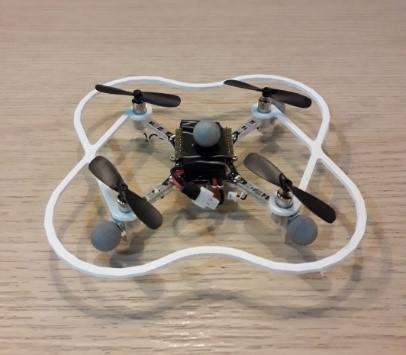
\includegraphics[width=5cm]{images/testbed/cf.jpg}
  \caption{The Crazyflie 2.1 miniature quadcopter with four motion-capture markers, expansion boards (not visible), and battery.}
  %\label{fig:marginfig}
\end{marginfigure}
 
The Crazyflie Drone has several advantages over other drones.

\begin{itemize}
    \item	\textbf{Autonomous Flight}. State estimation and trajectory planning are managed by the Crazyflie firmware. The operating procedure is simplified to sending setpoint commands from a remote PC. \cite{crazyflie_docs}
    \item	\textbf{Programmability}. At the moment of writing, there are two APIs known to send high-level commands to the drone. \cite{crazyflie_docs}
    \item   \textbf{Dimensions}. Due to our space constraints, a small, light  drone is preferable. Our payload of motion-capture markers brings the Crazyflie’s mass to 33 grams. 
    \item   \textbf{Reconfigurability}. The Crazyflie is easily assembled and maintainable. It is compatible with a range of sensor modules for different activities. \cite{crazyflie_docs} 
\end{itemize}
    %If a drone swarm is be densely packed, it causes downflowing air currents that disturb the stability in drone flight \cite{phan_hönig_ayanian_2018}. 
% \begin{figure*}[h]
%     \raggedright
%     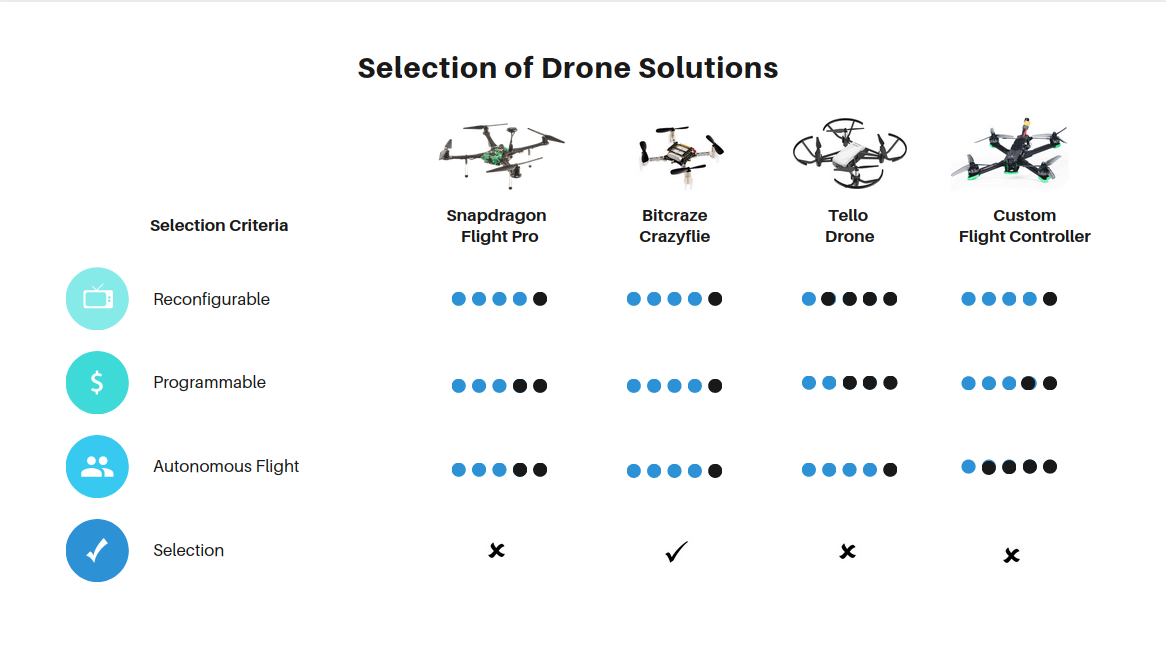
\includegraphics[width=12cm]{images/testbed/testbed_arch/drone-selection.png}
%     \caption{Overview of Selection Process.}
% \end{figure*}

\subsection{Flight Arena and Spatial Localization}
% [Optitrack] 
\begin{marginfigure}%
  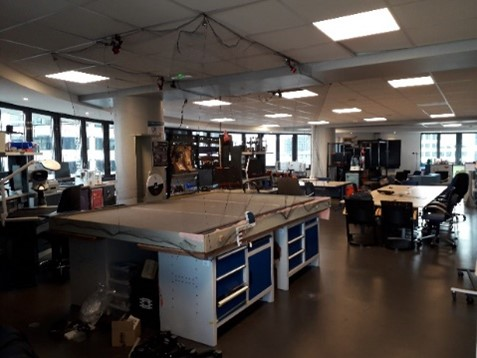
\includegraphics[width=5cm]{images/testbed/platform.jpg}
  \caption{The Motion Capture Table, net and Flex 13 cameras positioned above the platform.  }
  \label{fig:flight_arena}
\end{marginfigure}

\begin{marginfigure}
  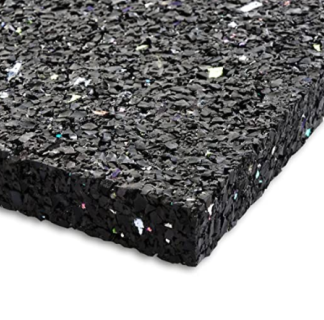
\includegraphics[width=5cm]{images/testbed/camera_layout/cork_material.png}
  \caption{Protective cork layer.}
  \label{fig:cork}
\end{marginfigure}


The Flight Area (Figure \ref{fig:flight_arena}) measures 3 x 2 meters, with a table-to-ceiling distance of 1.3m. In order to dampen the impact of falling drones, the table is layered with anti-vibration cork material (Figure \ref{fig:cork}). 

Optitrack \cite{optitrack} was adopted as the Motion Capture since the equipment was available in the laboratory. It is compatible with the swarm management solution of Section \ref{section:swarm}. Optitrack uses a Point Cloud reconstruction engine \cite{optitrack_docs}. That is, it triangulates two-dimensional points from camera images into coordinates in a three-dimensional space. For this purpose, four Flex 13 cameras are set up on the Flight Arena (as seen in Figure \ref{fig:flight_arena}).

The Flex 13 cameras \cite{optitrack_docs} are infrared cameras, and so they must have an unobstructed view of any tracked object. 

The exact positions of the cameras give a certain coverage of the Flight Arena. The next section determines how much of the Flight Arena is localized by the cameras.

\pagebreak
\subsection{Lightray Coverage Study}



We investigate how much of the flight arena is localized by the motion capture. The drones can only be flown in a space covered by the infrared cameras, therefore we perform a design study to maximize this flight space.


\subsubsection{Lightray Simulation}

A model is designed in Solidworks \cite{solidworks} to simulate the coverage of our cameras. Figure \ref{fig:45} simulates the camera coverage on a table the size of the Flight Arena.  
A key factor is the camera's pitch angle down from the horizontal. Figure \ref{fig:45} compares an orientation at 45° from the horizontal to one at 30 degrees.

\begin{figure*}[h]
    \raggedright
    %\hspace*{\fill}   % maximize separation between the subfigures
    \subfloat[Isometric view of 45deg rays]{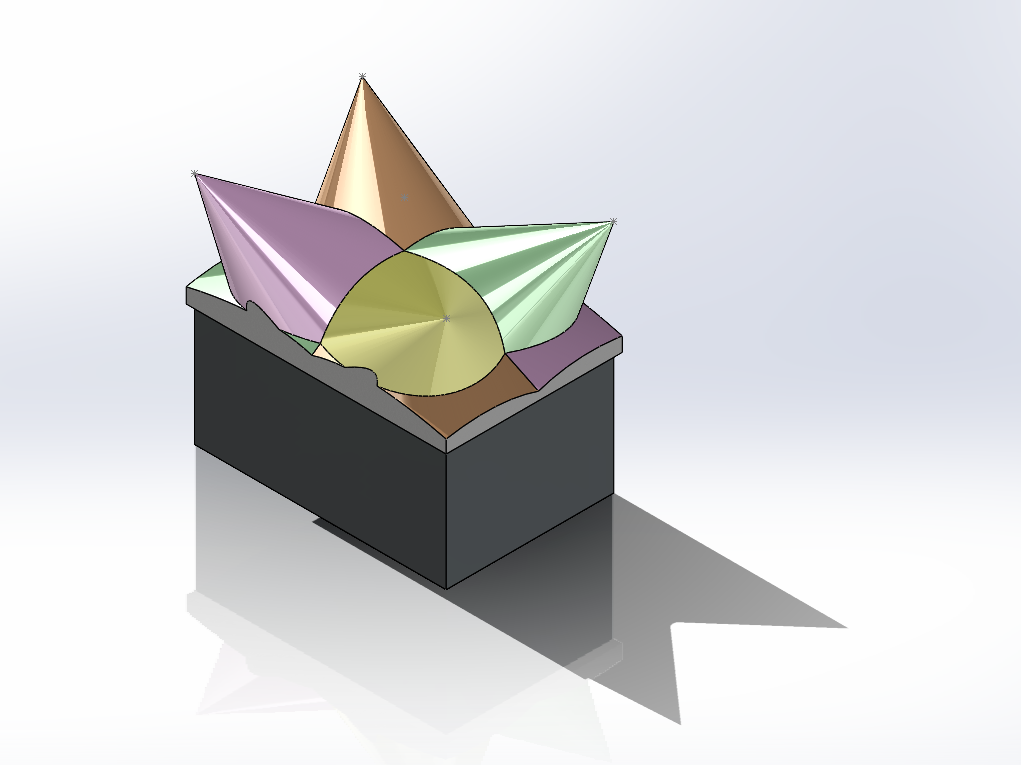
\includegraphics[height=4cm, width=5cm]{images/testbed/camera_layout/45_iso.PNG}}
    \subfloat[Isometric view of 30deg rays]{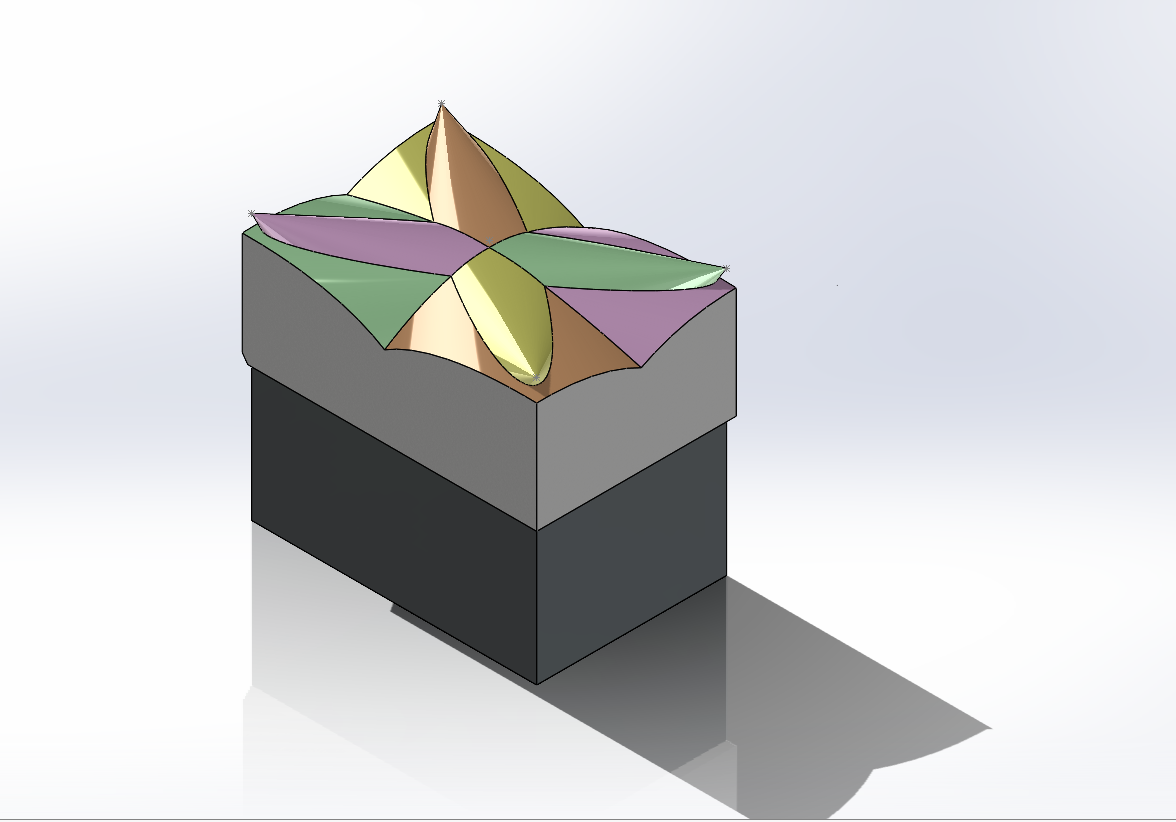
\includegraphics[height=4cm]{images/testbed/camera_layout/30_iso.PNG}}
    % \\
    % \subfloat[Frontview of 45deg rays]{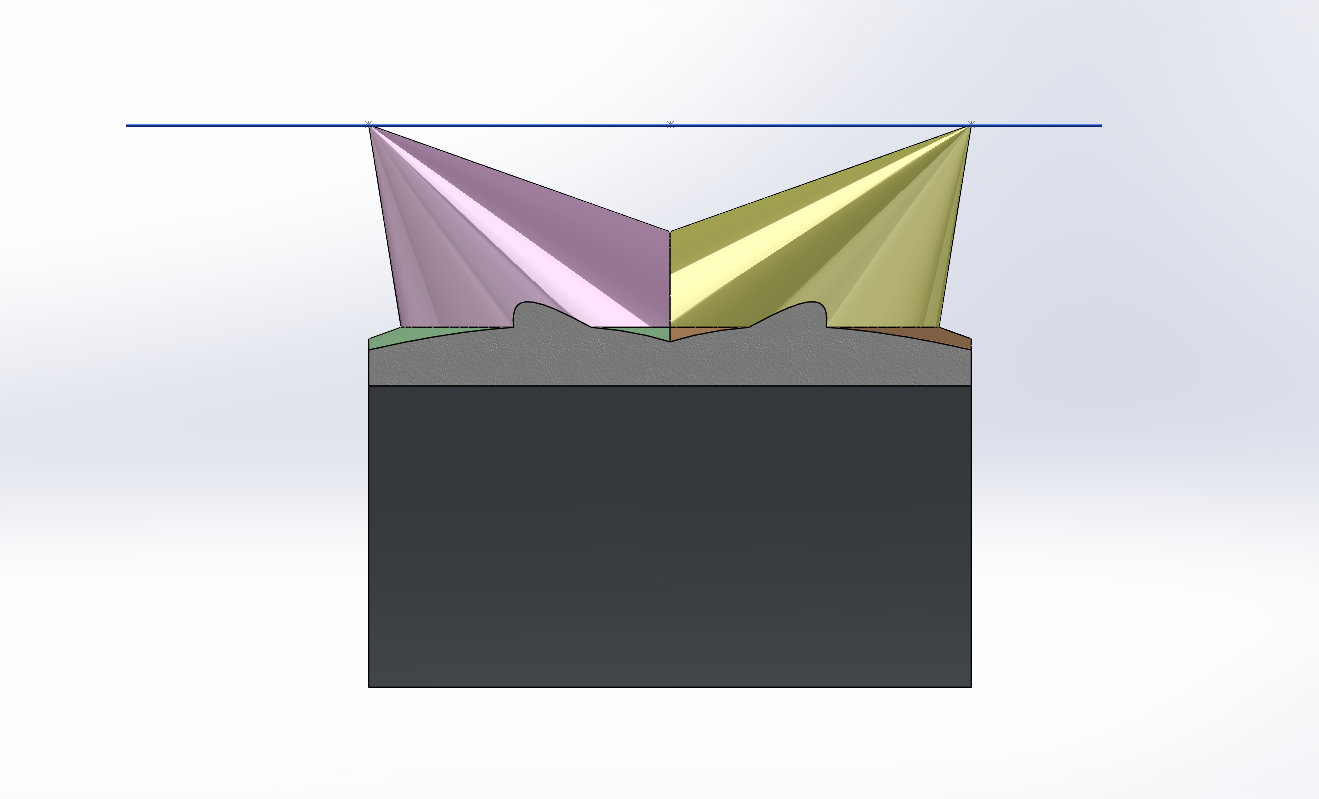
\includegraphics[height=4cm]{images/testbed/camera_layout/45_frontview.PNG}}
    % \subfloat[Sideview of 45deg rays]{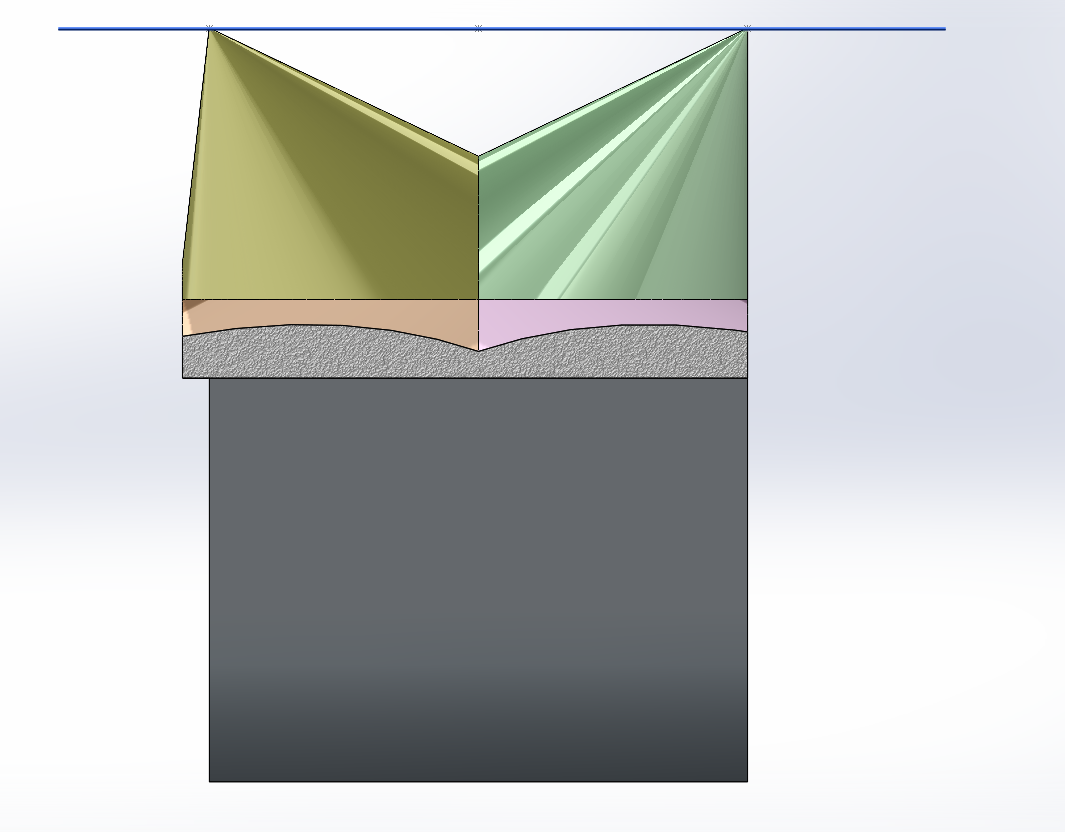
\includegraphics[height=4cm]{images/testbed/camera_layout/45_sideview.PNG}}
    \caption{Lightray simulation on the Table for 45° angle from the horizonta}
    \label{fig:45}
\end{figure*}

\begin{marginfigure}%[h]
    \raggedright
    %\hspace*{\fill}   % maximize separation between the subfigures
    \subfloat[Camera Ray]{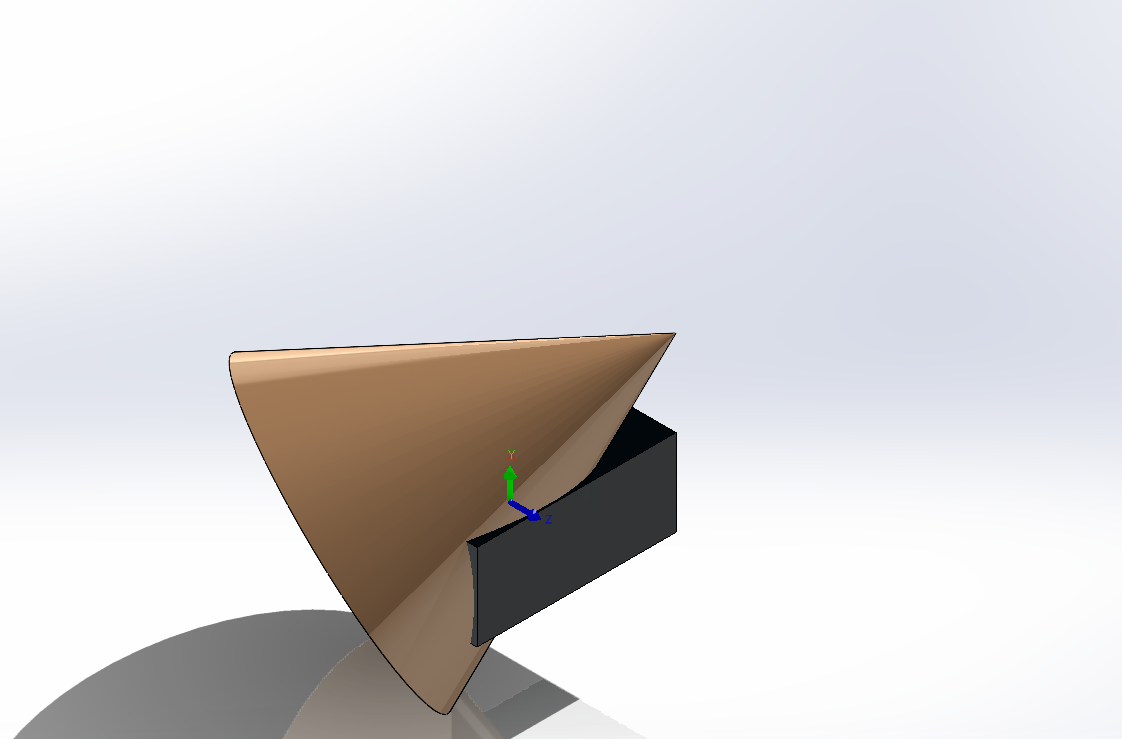
\includegraphics[height=2cm]{images/testbed/camera_layout/intersection/firstray.PNG}}
    \subfloat[4 camera rays]{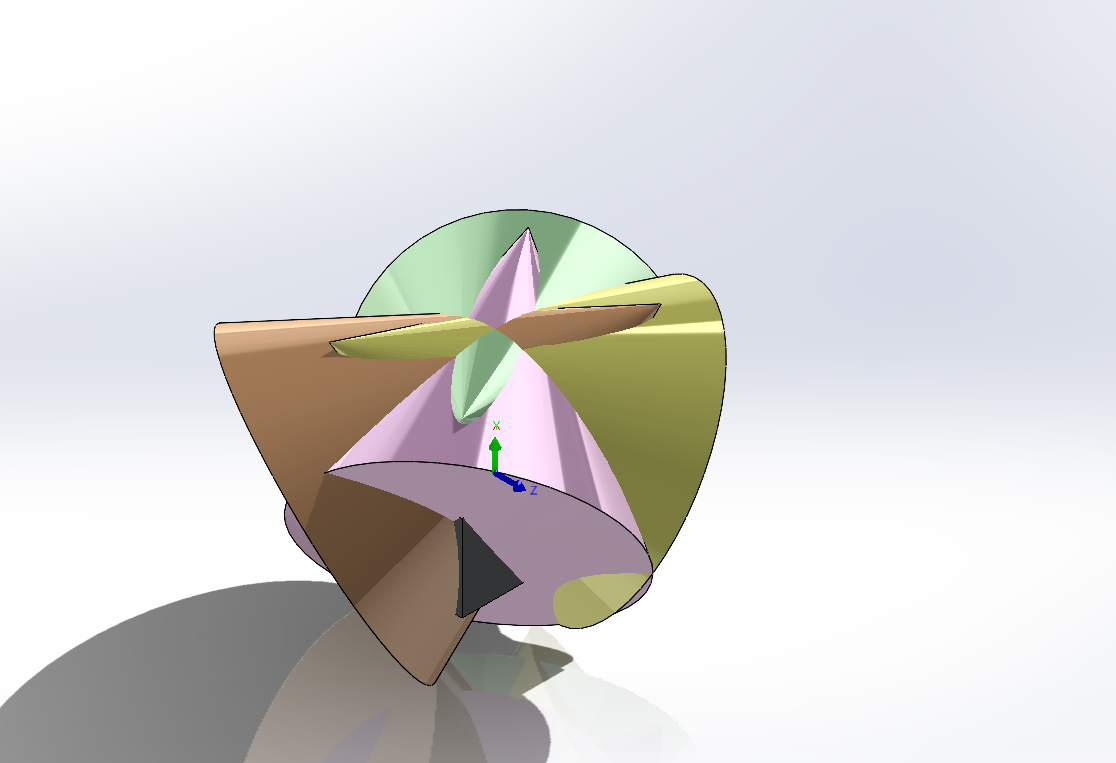
\includegraphics[height=2cm]{images/testbed/camera_layout/intersection/allrays.PNG}}
    \\
    \subfloat[Intersection Region]{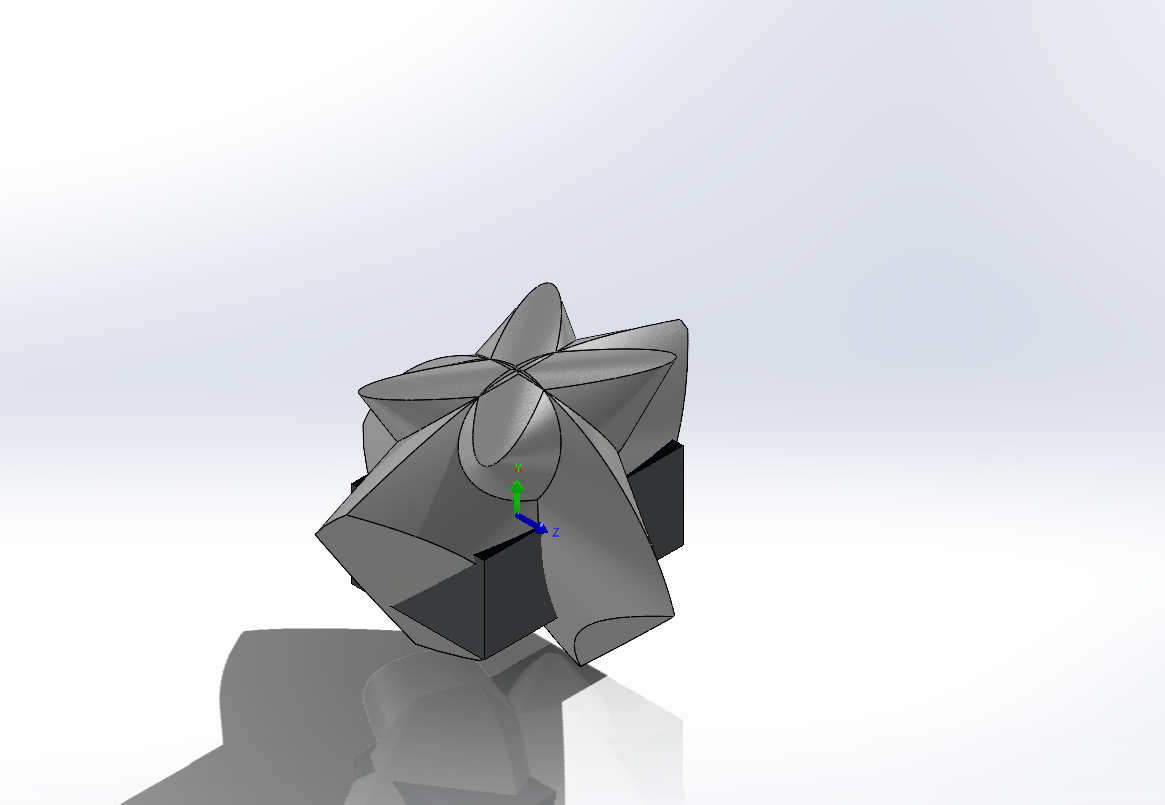
\includegraphics[height=2cm]{images/testbed/camera_layout/intersection/intersection.PNG}}
    \subfloat[Covered Volume ]{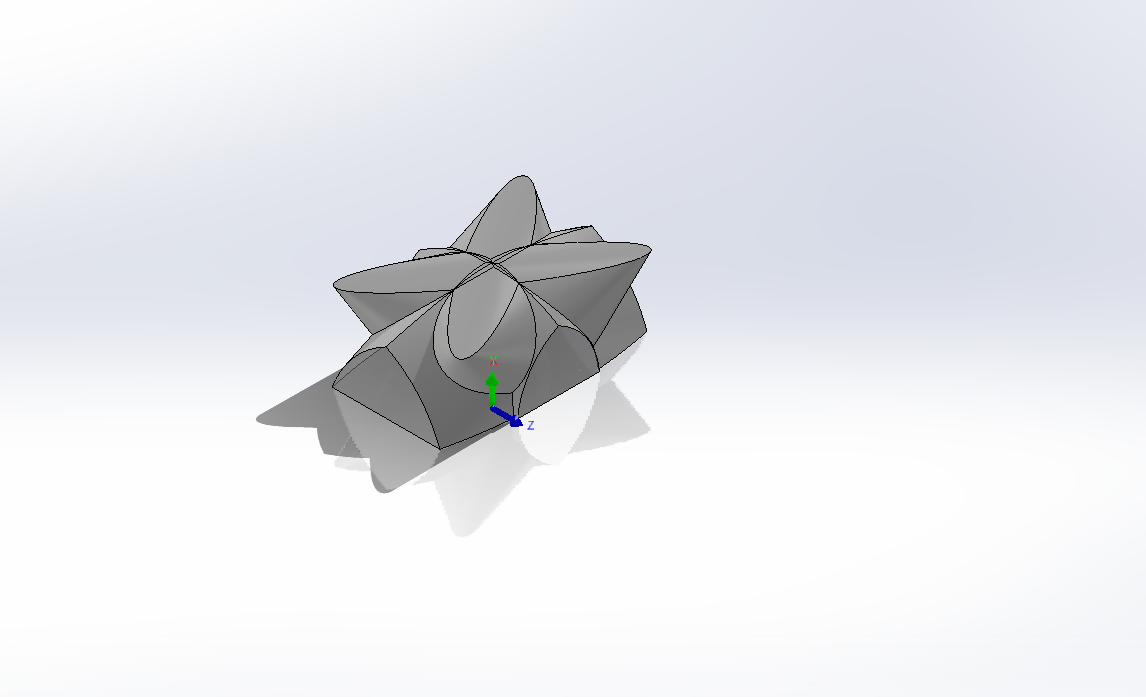
\includegraphics[height=2cm]{images/testbed/camera_layout/intersection/final.PNG}}
    \caption{Modelling the Coverage Volume}
    \label{fig:intersection_procedure}
\end{marginfigure}

The coverage percentage is determined as the volume of space localized by the flight cameras over the total usable volume above the Flight Arena. Figure \ref{fig:intersection_procedure} shows the modelling process of ray coverage volumes. The design requirements are as follow:
\begin{itemize}
\item The cameras are placed above the table corners. within the net region so as to have a clear view of the drones when the net is lowered
\item There are a total of 4 cameras available during motion capture installation. The flight space measures 3×2×1.3 m.
\item Flex 13 cameras have a 56° field of view, and this is replicated in simulation (Figure \ref{fig:intersection_procedure}). 
\item In order to triangulate a position, the motion capture requires a minimum of 2 rays to intersect \cite{optitrack_docs}.
\end{itemize}

These volumes can then be determined in Solidworks using its Volumetric Tool \cite{solidworks_docs}.
% \begin{figure*}[!h]
%     \raggedright
%     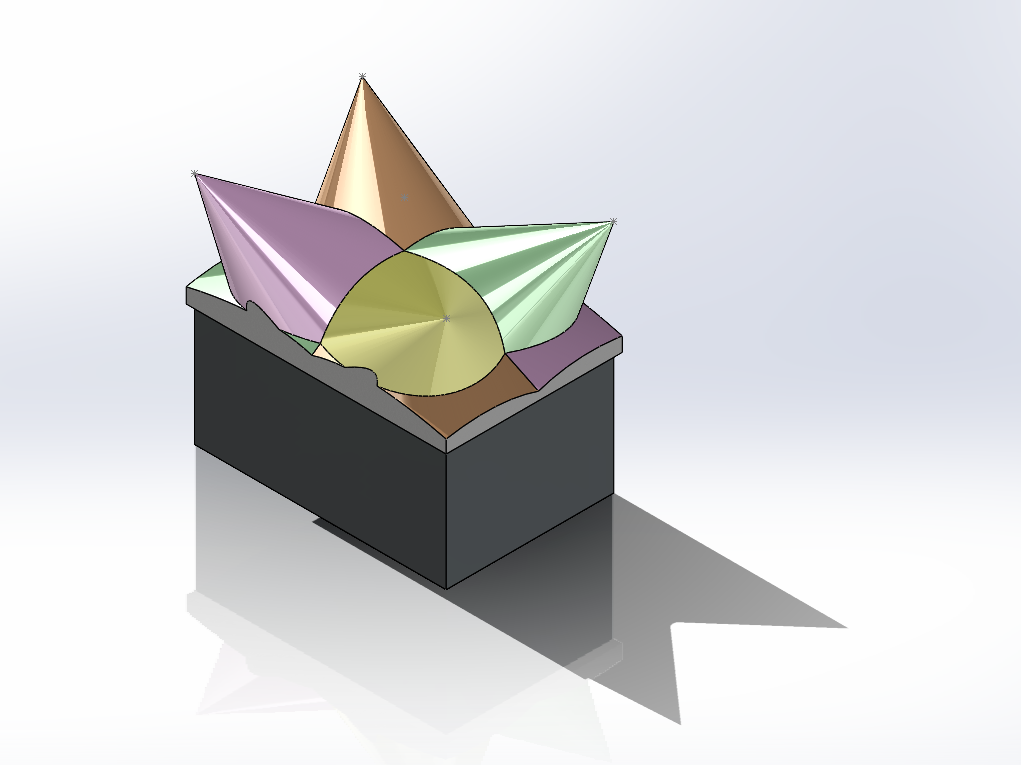
\includegraphics[width=3cm]{images/testbed/camera_layout/45_iso.PNG}
%     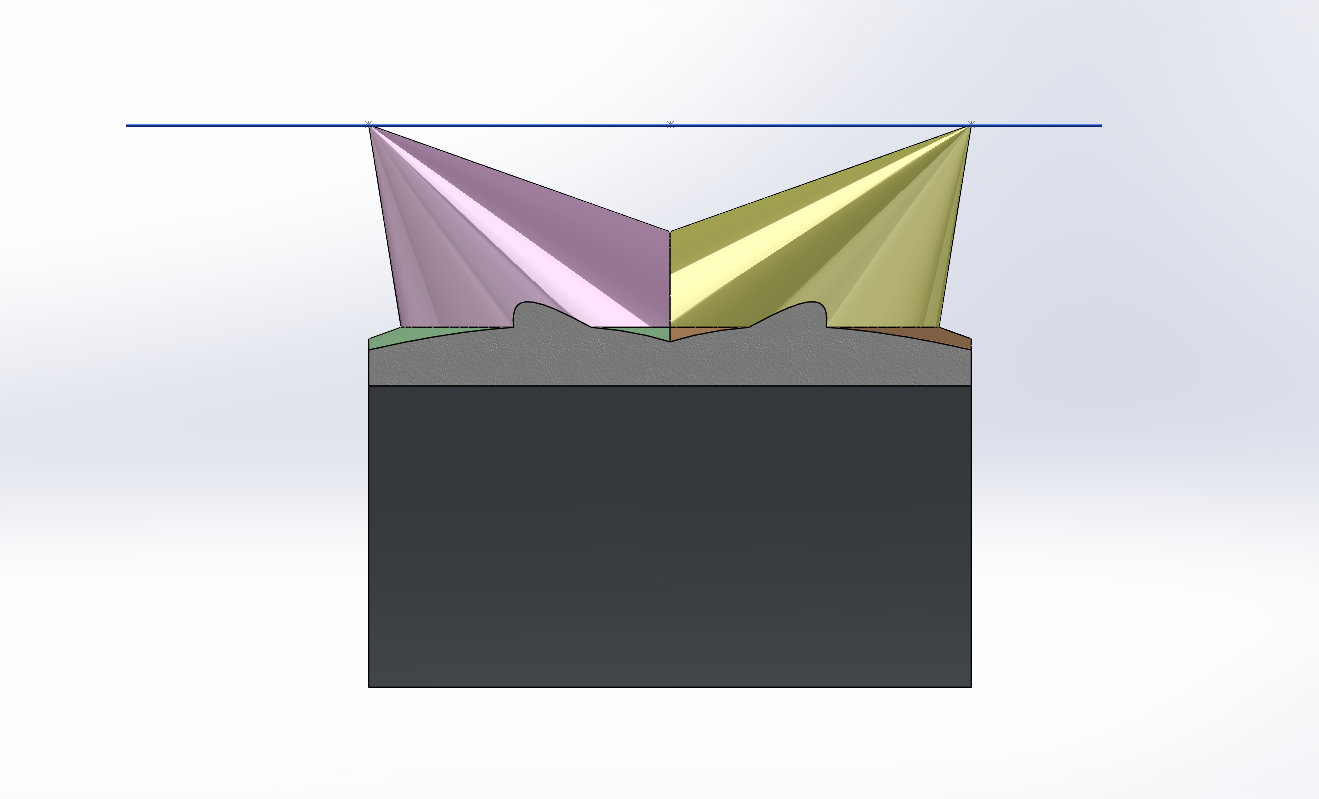
\includegraphics[width=3cm]{images/testbed/camera_layout/45_frontview.PNG}
%     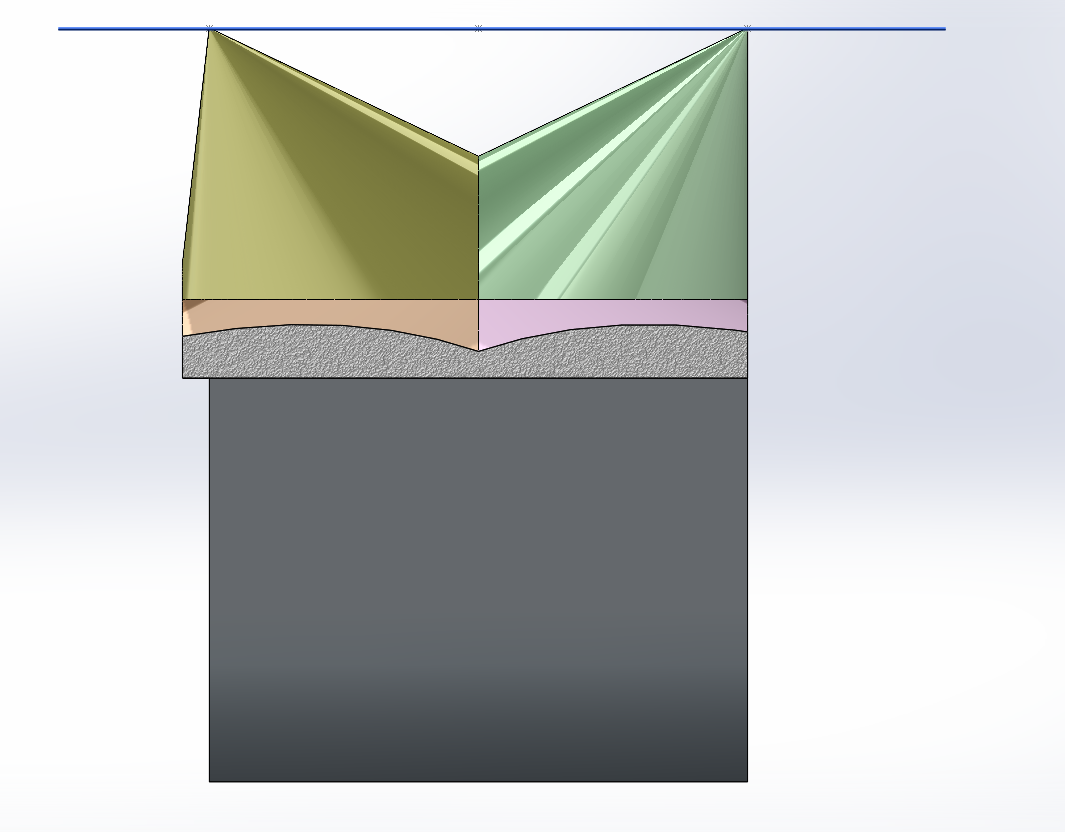
\includegraphics[width=3cm]{images/testbed/camera_layout/45_sideview.PNG}
%     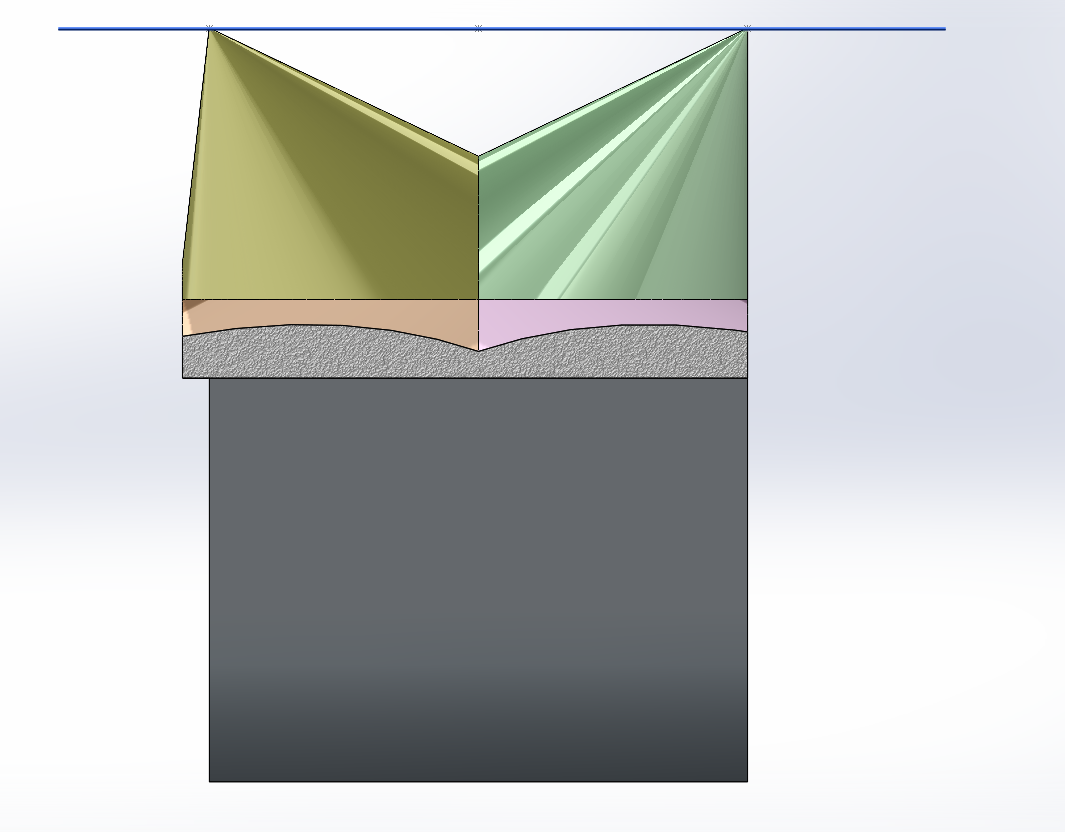
\includegraphics[width=3cm]{images/testbed/camera_layout/45_sideview.PNG}
%     \caption{Lightray simulation on the Table for 45° angle from the horizontal}
%     \label{fig:45}
% \end{figure*}
For a pitch angle of 30$^o$, The volumes of the flight space and of the intersection area above, are respectively of 7.8 $m^2$ and 6.134 $m^2$. As a result, we determine that the usable region for flight is 78.64\% of the 3×2×1.3 m flight space. This demonstrates that 20\% of the flight space is unusable. This is not surprising, considering that 4 cameras are directly above the table and constrained by the netting.



% 1. At corners
% 15 deg. 6 970 142 481.03 cubic millimeters
% 20 deg. 7 014 173 181.97 cubic millimeters
% 25 deg. 6 804 720 310.30 cubic millimeters 
% 30 deg. 4 855 500 995.33 cubic millimeters
% 35 deg. 5 006 693 602.87 cubic millimeters
% 40 deg. 3 747 076 773.66 cubic millimeters


\pagebreak
\subsubsection{Coverage Optimisation Study}

The camera's pitch angle is varied to determine the point of optimal coverage. Figure \ref{fig:volumes} shows the volumes generated during the study.

\begin{figure*}[!h]
    \raggedright
    \hspace{1cm}\subfloat[With pitch of $20^o$]{\hspace{-1cm}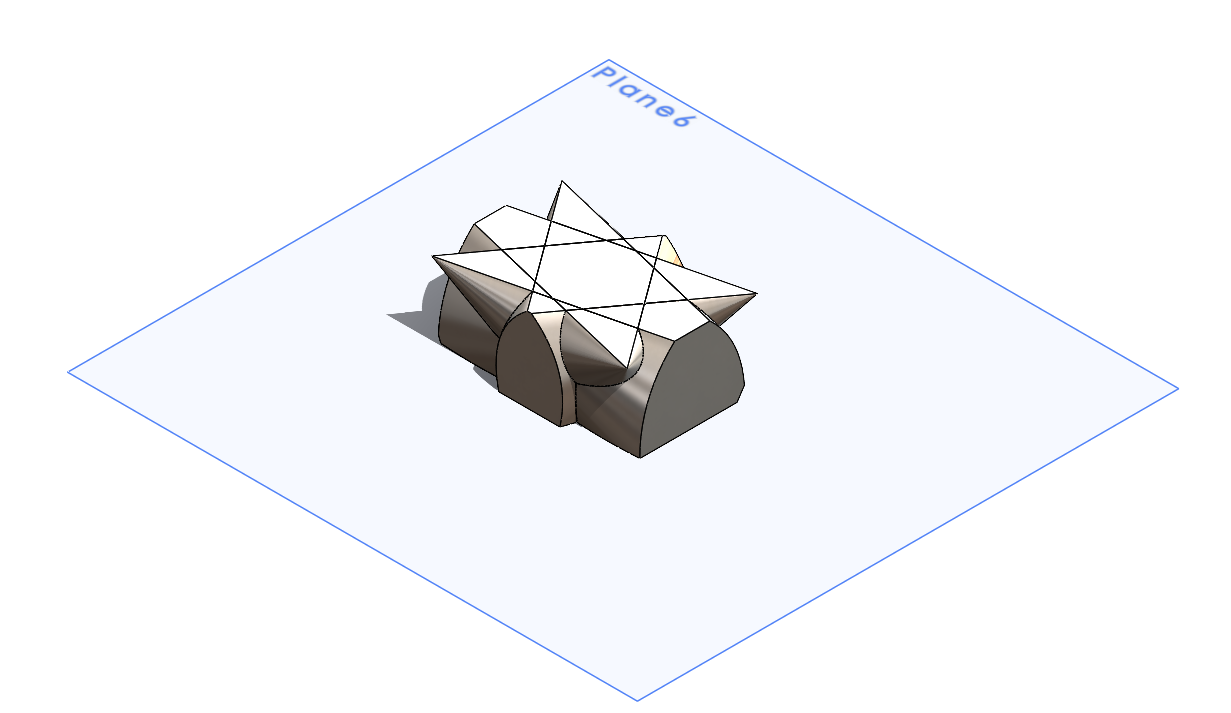
\includegraphics[height=3.8cm]{images/testbed/camera_layout/corner_20deg.PNG}
    }
    \hspace{1cm}\subfloat[With pitch of $25^o$]{\hspace{-1cm}
    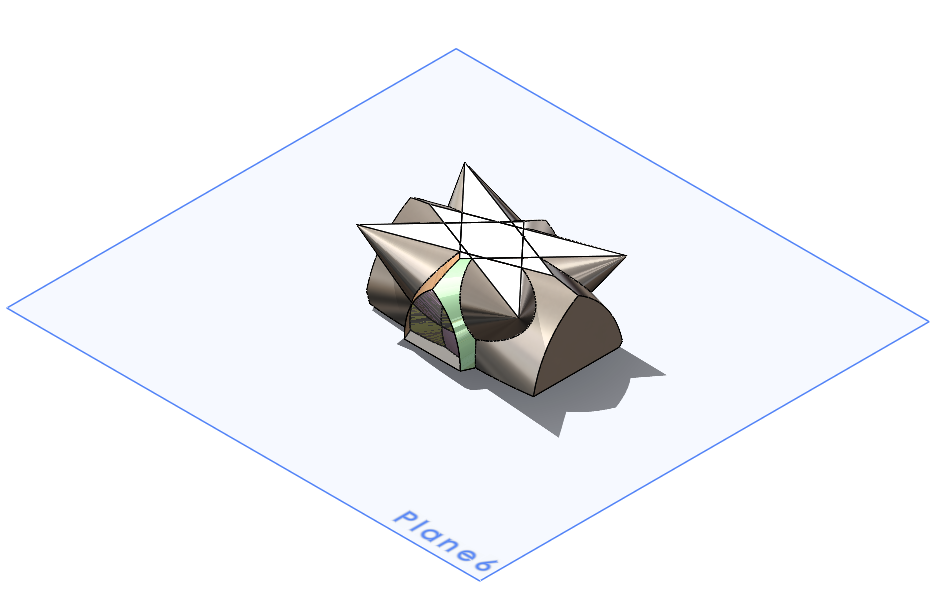
\includegraphics[height=3.8cm]{images/testbed/camera_layout/corner_25deg.PNG}
    }\\
    \hspace{1cm}\subfloat[With pitch of $30^o$]{\hspace{-1cm}
    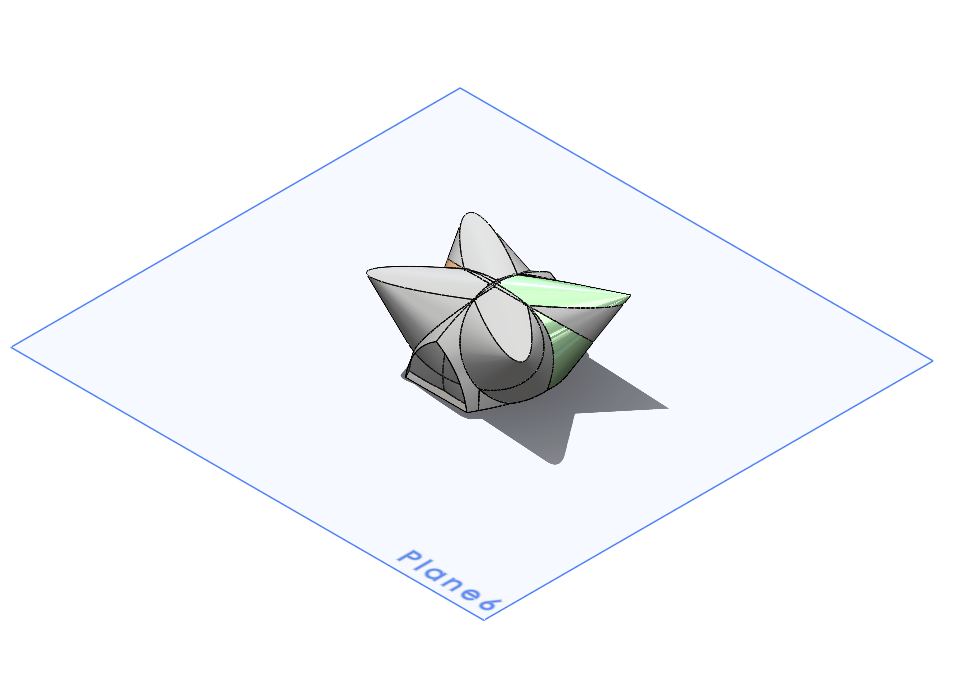
\includegraphics[height=4cm]{images/testbed/camera_layout/corner_30deg.PNG}
    }
    \hspace{1cm}\subfloat[With pitch of $35^o$]{\hspace{-0.8cm}
    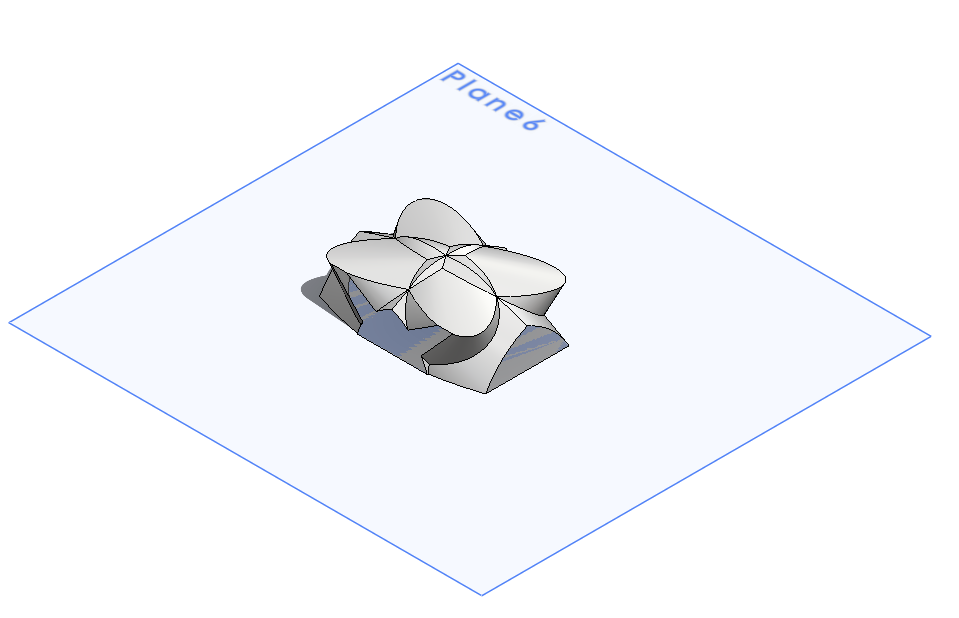
\includegraphics[height=4cm]{images/testbed/camera_layout/corner_35deg.PNG}
    }\\
    \caption{Lightray simulation for Intersection of any 2 lightrays.}
    \label{fig:volumes}
\end{figure*}


The study has two parts. The first study varies by increments of 5$^o$, in order to determine the range of volume maxima. The second study finetunes by increments of 1$^o$, with the help of a Solidworks Design Study \cite{solidworks_docs}. This simulation tool is used to generate volumes automatically. It has trouble generating volumes if the angle increments are too large, therefore the first study is done manually.

\begin{table*}[!h]
  \raggedright
  \footnotesize
    \subfloat[Finding Local Maxima with Manual Study]{
        \begin{tabular}{lcccl}
          \toprule
          Pitch                      & Volume & \% & Max \\
          (deg)                      & ($mm^3$) & Covered & Range \\
    
          \midrule
          
          
          10                 & 6 607 805 800.35    & 84.7154 &  \Circle \\
          15                 & 6 970 142 481.03    & 89.3608 &  \CIRCLE \\
          20                 & 7 014 173 181.97    & 89.9253 &  \CIRCLE \\
          25                   & 6 804 720 310.30      & 87.2400 & \CIRCLE  \\
          30             & 4 855 500 995.33   & 62.2500 &  \Circle  \\
          35             & 5 006 693 602.87 & 64.1884 &  \Circle \\
          40             &  3 747 076 773.66 & 48.0394 &  \Circle \\
          \bottomrule
        \end{tabular}
    }
    \subfloat[Finetuning with Automatic Design Study]{
        \begin{tabular}{lcccl}
          \toprule
          Pitch                      & Volume   & \%        & Max \\
          (deg)                      & ($mm^3$) & Covered & Range \\
          
          \midrule
          16                 & 7007549683.27    &89.8404  &  \Circle \\
          17                   & 7034381844.70      &90.1844 & \Circle  \\
          18             & 7050625519.44   &90.3926 &  \CIRCLE  \\
          19             & 7056144612.83 &90.4634 &  \CIRCLE \\
          20             &  7014172714.71 &89.9253 &  \CIRCLE \\
          21             &  6999358686.15 &89.7354 &  \Circle \\
          22             &  6972124192.42 &89.3862 &  \Circle \\
          \bottomrule
        \end{tabular}
    }
  %\end{flushleft}
  \caption{Results of Coverage Optimisation Study.}
  \label{tab:coverage_study}
\end{table*}
Through these studies, the coverage volume was increased from 78.64\% by \+11.31\% up to 89.95\%, and by \+0.51\% to \Copy{flight_arena_localized}{90.46\%}. This demonstrates that about 10\% of the flight space is still out of reach. While the netting constraint forces the cameras to have this inconvenience, the study could be further optimised by varying the yaw angle of the cameras and moving them away from the corners.

% \begin{figure*}[h]
%     \raggedright
%     %\hspace*{\fill}   % maximize separation between the subfigures
%     \subfloat[Camera ray with 56deg field of view]{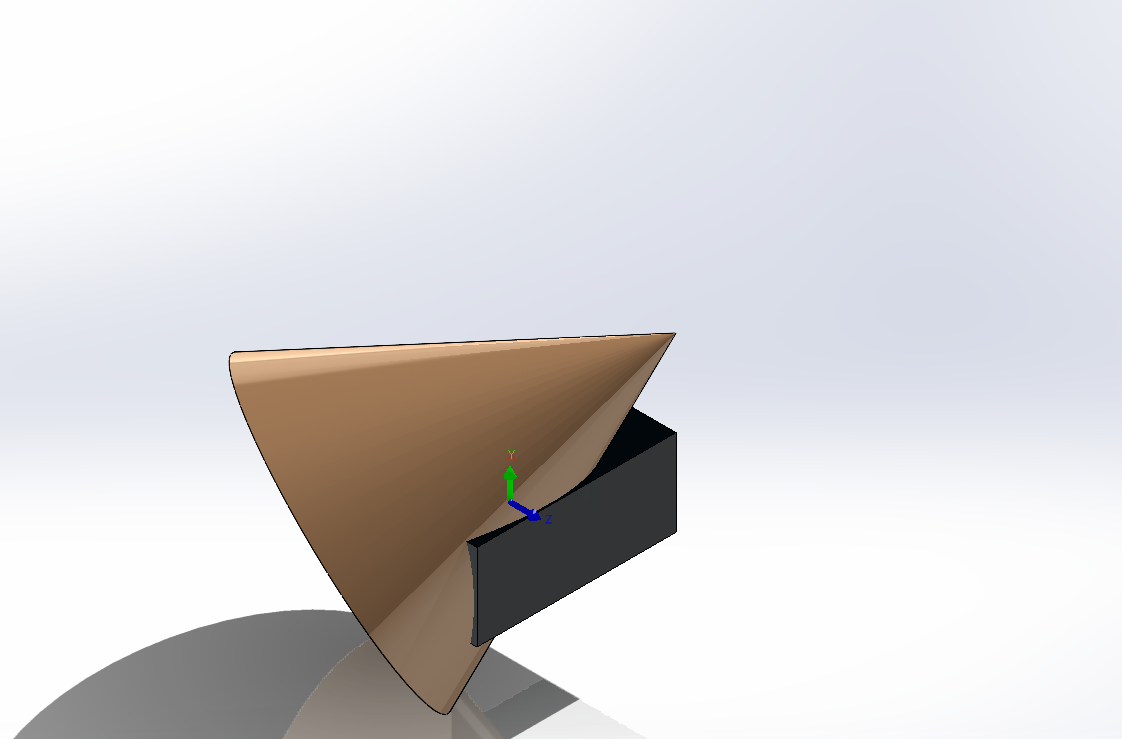
\includegraphics[height=3cm]{images/testbed/camera_layout/intersection/firstray.PNG}}
%     \subfloat[All 4 intersecting rays]{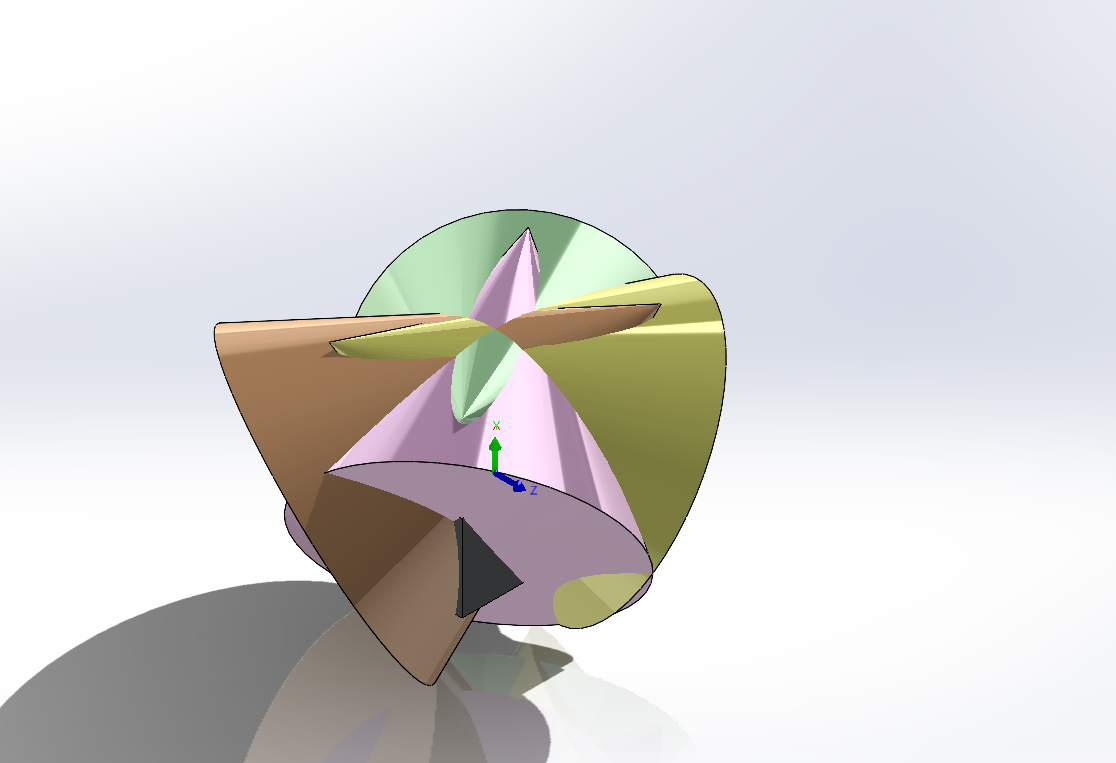
\includegraphics[height=3cm]{images/testbed/camera_layout/intersection/allrays.PNG}}
%     \\
%     \subfloat[Intersection of any 2 rays]{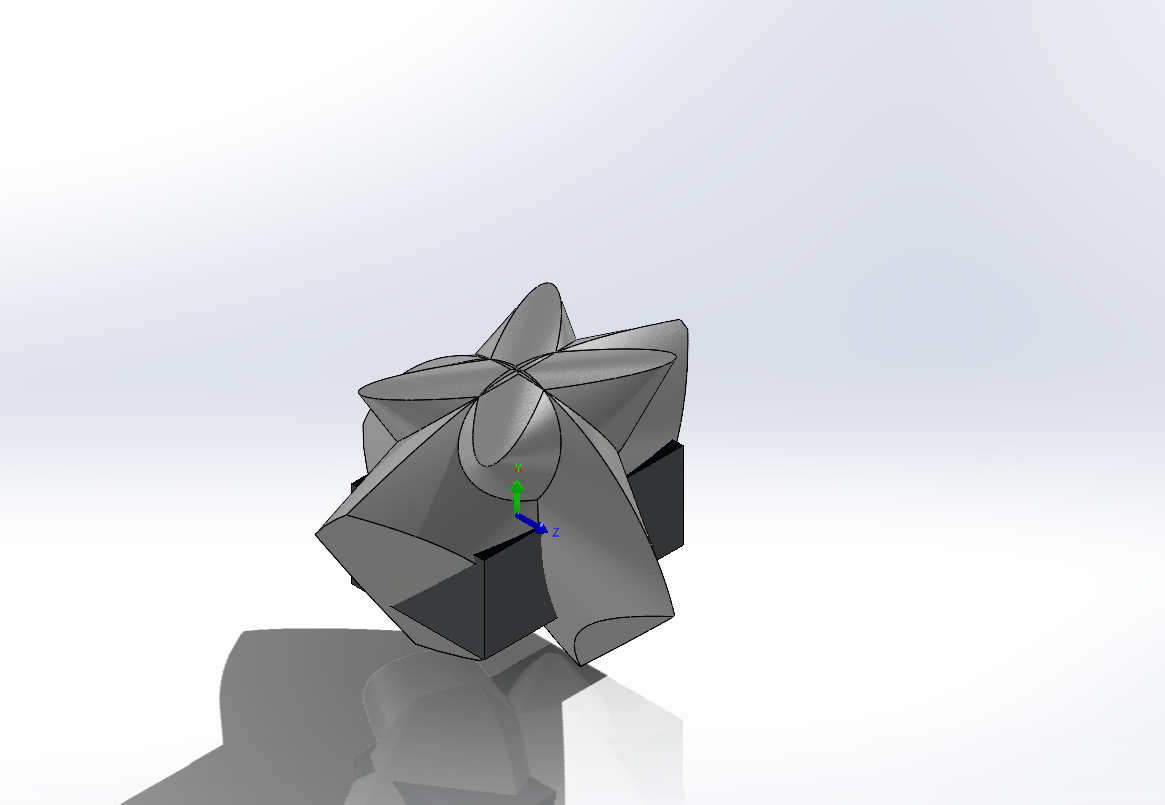
\includegraphics[height=3cm]{images/testbed/camera_layout/intersection/intersection.PNG}}
%     \subfloat[Intersection volume above table]{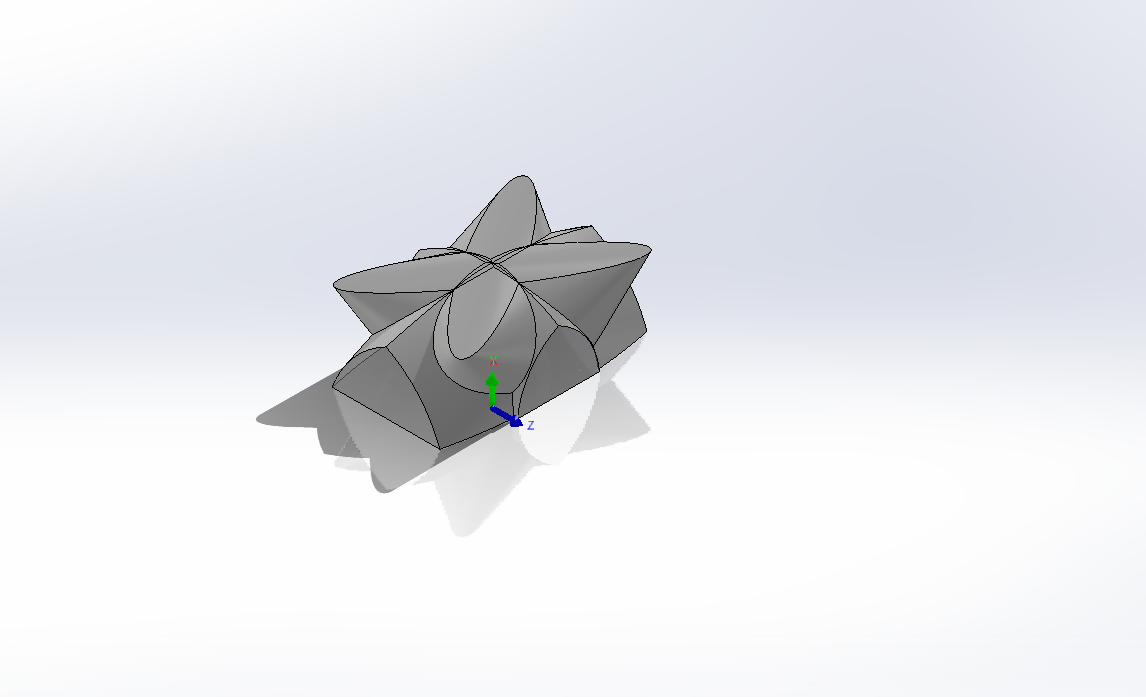
\includegraphics[height=3cm]{images/testbed/camera_layout/intersection/final.PNG}}
%     \caption{Determining the intersection area of lightrays}
%     \label{fig:intersection_procedure}
% \end{figure*}
% 15 | 6970142497.90 cubic millimeters
% 16 | 7007549683.27 cubic millimeters
% 17 | 7034381844.70 cubic millimeters
% 18 | 7050625519.44 cubic millimeters
% 19 | 7056144612.83 cubic millimeters
% 20 | 7014172714.71 cubic millimeters
% 21 | 6999358686.15 cubic millimeters
% 22 | 6972124192.42 cubic millimeters
% 23 | 6931446377.86 cubic millimeters


% EXACT CALCULATION 
% 6133948743.46/7800000000.00 = 0.7864
\pagebreak
\subsection{Flight Stability Tests}

Tests of the stability of robotic systems are routinely performed to measure their robustness to external forces. This is a key challenge in drone development \cite{crazyflie_docs}, where a drone maintains dynamic stability by counterbalancing six directions of freedom, as opposed to two for wheeled systems in static stability. 

\begin{marginfigure}%
  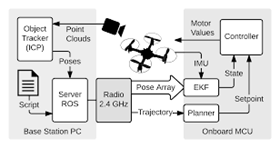
\includegraphics[width=6cm, center]{images/testbed/controlloop_bw.png}
  \caption{Overview of the Crazyswarm Control Loop, as per the Crazyswarm official documentation (August 2021) \cite{crazyswarm_docs}}
  %\label{fig:marginfig}
\end{marginfigure}

The Crazyswarm ecosystem \cite{crazyflie_docs} makes use of a position and rate controller for each drone in its swarm. This means that a setpoint is sent to each drone separately, each correcting their current pose towards the setpoint. The streaming setpoints are broadcasted from one or more antennas. As the number of drones in the swarm increases, they receive less frequent broadcasts from the antenna \cite{preiss_hönig_sukhatme_ayanian_2017}.

The purpose of this test is to determine the response of the drone's position and angle controllers to the natural disturbance during hovering. This experiment investigates the effect of antenna distance and interference on drone flight. With multiple drones to a single antenna, we evaluate if the system demonstrates any performance limits. 

\subsubsection{Hypothesis}
The hypothesis is as such: the error in drone pose will correlate with the distance of the drones from the antenna. 

\subsubsection{Prediction}
A hover stability test is a good measure of system performance since it requires quick readjustments of the drone to counter natural disturbances during hovering. In \cite{experimental_tuning}, \citename{experimental_tuning}{author} determine the performance of their flight controller by comparing the attitude of the drone in relation to the demanded null value of angular rotations. In contrast, our input is a setpoint. The output is a set of translation and rotational angles relative to a demanded null value for translation and rotation. This output is graphed as a deviation over time. The shape of the response charts are associated with flight stability over time.


\subsubsection{Experiment Methodology}
\begin{marginfigure}%[!h]
    \raggedright
    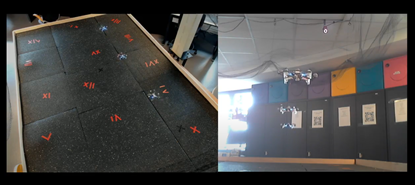
\includegraphics[width=5cm]{images/chore_pictures/3drones/pic.png}
    \caption{View of the Flight Arena during the 2 Drone Hover experiment.}
\end{marginfigure}
 Hover stability is examined on the Flight Arena. The telemetry recording and external video cameras are programmed to launch with the swarm control interface. Three drones are hovered in the Flight Arena at an altitude of around 1 m.  It was possible to record a 20-s long autonomous flight during which the flight controller attempted to stabilize the quadcopter. During that time, the quadcopter remained within a radius of two meters from its takeoff location. 

\textbf{Constraints}: In preparation for the flight, each of the three drones are inspected for minimal positional displacement of less than (1cm + 0.01 rad). This ensures fully functional position controllers for the drones. 
% The recorded position of these drones is analyzed for further insight \footnote{Data available: https://drive.google.com/drive/folders/1hh6v1r74IvHczOsqgnFKYhRzEkGcKciW?usp=sharing}.\\

% \underline{Logging Flight Data}\\
% Data is logged at 200 Hz, in particular the /tf2 node containing the recorded positions of all three drones.

% \underline{System Node Graph}\\
% Of particular interest is the drone control loop.

% \underline{Drone layout}\\
% 3 drones are aligned along an axis on the Flight Arena.



% 3D VIEW DOES NOT FIT WITH THE REST.
%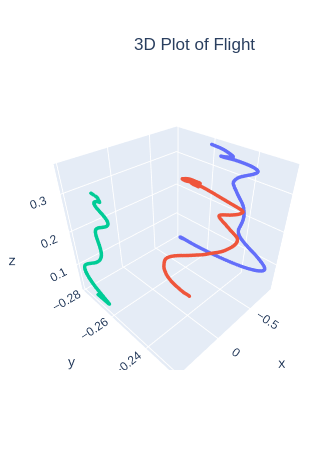
\includegraphics[width=3.5cm]{images/chore_pictures/3drones/3d.png}
\pagebreak

\subsubsection{Results}


The flightpaths of the three drones are plotted alongside . The topview and the sideview are featured below.


\begin{figure*}[!h]
    \raggedright
    \hspace{2cm}
    \subfloat[X translations]{\hspace{-2cm}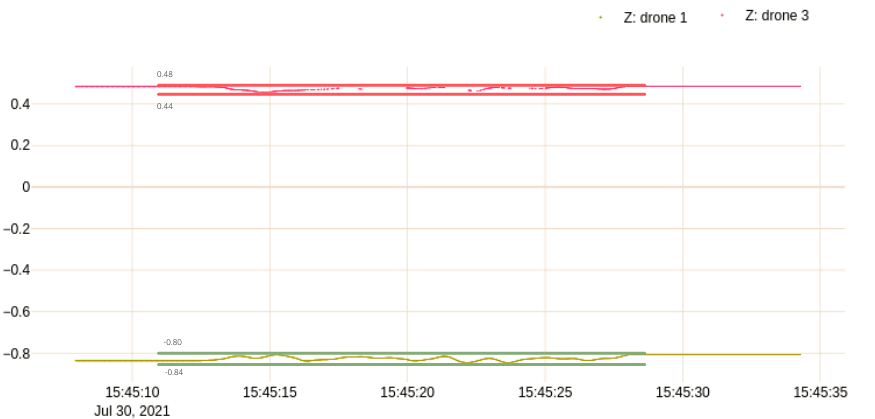
\includegraphics[width=6cm]{images/chore_pictures/3drones/x_translations_ann.png}}
    \hspace{2cm}\subfloat[Y translations]{\hspace{-2cm}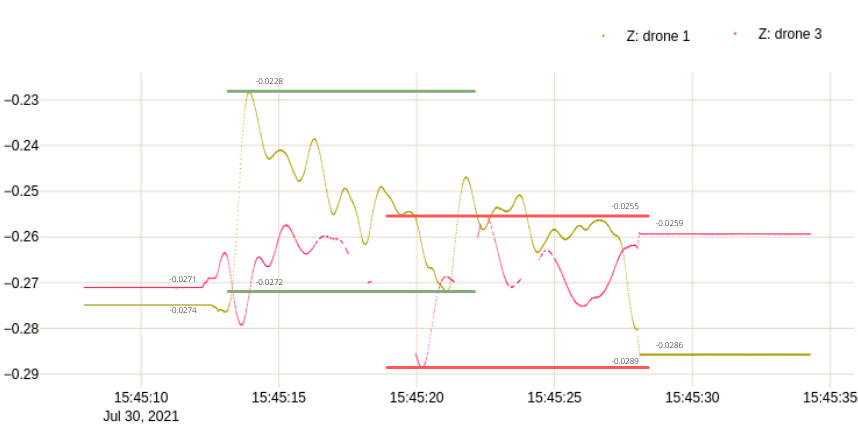
\includegraphics[width=6cm]{images/chore_pictures/3drones/y_translations_ann.png}}\\
    \hspace{2cm}\subfloat[Z translations]{\hspace{-2cm}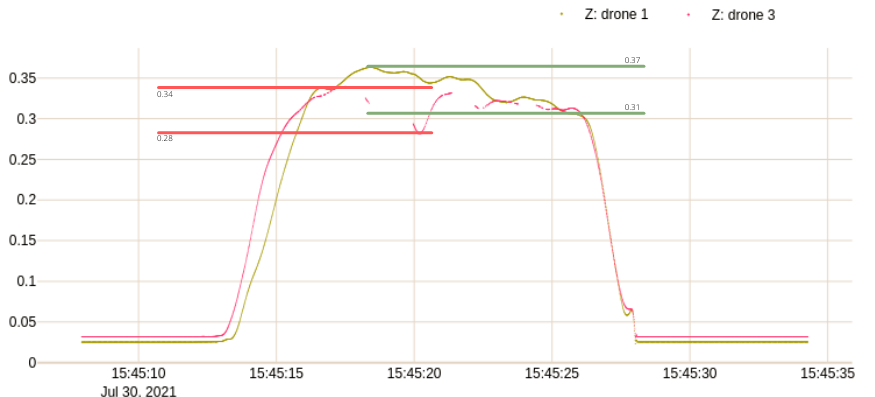
\includegraphics[width=6cm]{images/chore_pictures/3drones/z_translations_ann.png}}
    \hspace{1cm}\subfloat[Roll, pitch and yaw rotations]{\hspace{-1cm}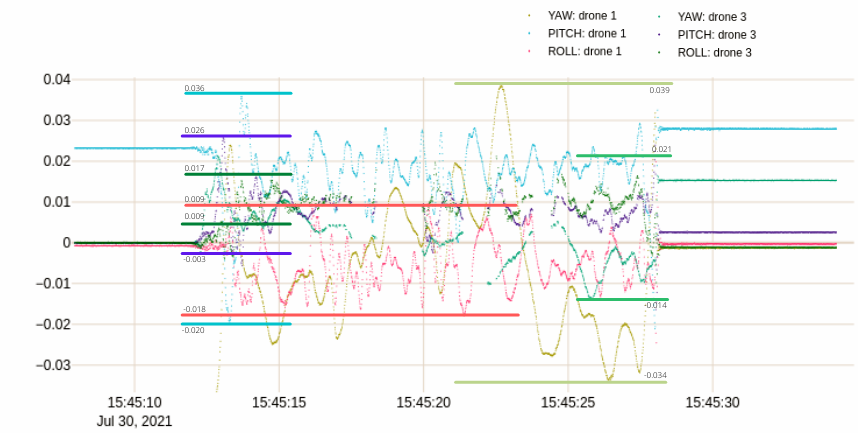
\includegraphics[width=6cm]{images/chore_pictures/3drones/anglerates_ann.png}}
    \caption{Hover Experiment: Stability Tests on Flight Arena.}
\end{figure*}

\begin{marginfigure}%
  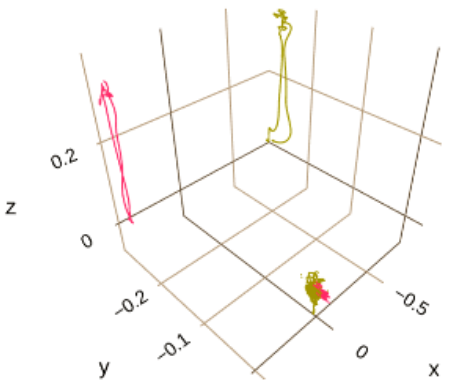
\includegraphics[width=4.5cm]{images/chore_pictures/3drones/3dplot_paths_inv.png}
  \caption{3D Plot of 2 Drone Hover.}
  \label{fig:hover_2drones}
\end{marginfigure} 

The flightpaths are smooth and generally show very minimal jerking. There are very little discontinuities, attesting to a continuous localization process. 

\begin{table*}[h]
  \raggedright
  \footnotesize%

    \begin{tabular}{lccccccl}
    
      \toprule
      \textbf{Criteria}                      & \textbf{Drone 1} &  &  & \textbf{Drone 2} &  & \\
                                    & Min & Max & Range & Min & Max & Range \\
      \midrule
      X                 & -0.84 & -0.80 & 0.04    & 0.44 & 0.48 &  0.04 \\%& \CIRCLE \CIRCLE \CIRCLE \CIRCLE \Circle & \CIRCLE \CIRCLE \Circle \Circle \Circle  \\
      y                 & -0.0272 & -0.0228 & 0.0044    & -0.0289 & -0.0255 & 0.0034 \\%& \CIRCLE \Circle \Circle \Circle \Circle & \CIRCLE \CIRCLE \CIRCLE \CIRCLE \Circle  \\
      Z                   & 0.31 & 0.37 & 0.06      & 0.28 & 0.34 & 0.06  \\%& \CIRCLE \CIRCLE \CIRCLE \Circle \Circle & \CIRCLE \CIRCLE \Circle \Circle \Circle \\
      Roll             & -0.018 & 0.009 &  0.027 & 0.009 & 0.017 & 0.008    \\%& \CIRCLE \CIRCLE \CIRCLE \CIRCLE \Circle & \CIRCLE \Circle \Circle \Circle \Circle\\
      Pitch           & -0.020 & 0.036 & 0.056  & -0.003 & 0.026 &  0.029 \\%& \CIRCLE \CIRCLE \CIRCLE \CIRCLE \Circle & \CIRCLE \Circle \Circle \Circle \Circle\\
      Yaw             & -0.034 & 0.039 &  0.073 & -0.014 & 0.021 &  0.035 \\%& \CIRCLE \CIRCLE \CIRCLE \CIRCLE \Circle & \CIRCLE \Circle \Circle \Circle \Circle\\
      \toprule
      
      Selection                     &&&  \ding{55} &&&  \ding{51} \\%&  \ding{55} &  \ding{55} \\
      \bottomrule
    \end{tabular}
  %\end{flushleft}
  \caption{Stability Comparison of two Drones.}
  \label{tab:stability_comparison}
\end{table*}

Drone 2 has less variation in both translations and rotations than Drone 1. This is confirmed in Table \ref{tab:stability_comparison}. Drone 2 is more stable in this test than Drone 1. The sample hover error is \Copy{sample_hover_error}{$\pm 72.24$ \text{mm} $\pm 0.096$ \text{rad}}.
% >>> math.sqrt((0.04**2)+(0.0044**2)+(0.06**2))
% 0.07224513824472897
% >>> math.sqrt((0.027**2)+(0.056**2)+(0.073**2))
% 0.09588534820294496
% \begin{figure*}[!h]
%     \raggedright
%     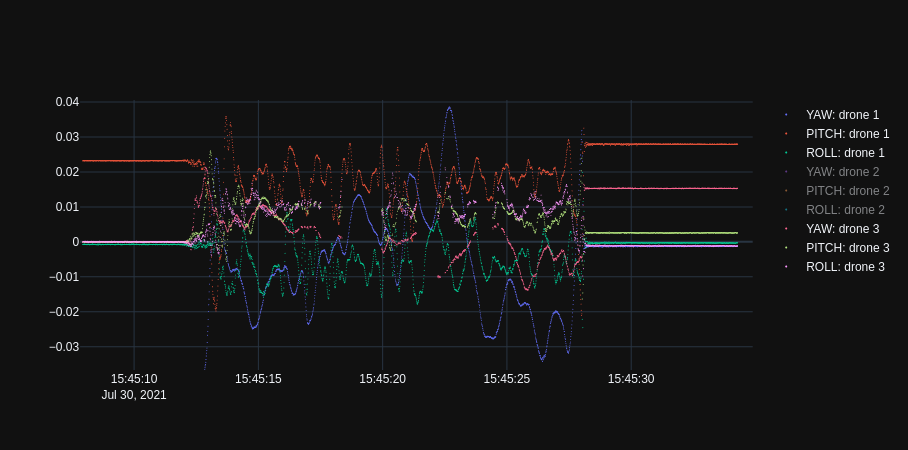
\includegraphics[width=11cm]{images/chore_pictures/3drones/anglerates.png}
%     \caption{Hover Experiment: Pitch, Yaw and Roll of the two drones.}
% \end{figure*}

The discrepancy between the two drones could be attributed to a number of factors.  This work may be improved with a second test, where the two drones' positions are inversed. All in all, the flight is substantially accurate, with a peak translation of 6cm.

\subsubsection{Conclusion of Test}
% stability_test_evaluation_conclusion}
Drone 2 is further from the arena and exhibits more stability. The drone that is furthest from the antenna does not have more pose error, and the hypothesis is rejected.
\pagebreak
\section{Software Environment}\label{section:software}


\subsection{Modules involved in Software Environment}

This section is a brief mention of all the platforms, systems, services, and processes the software environment would depend on.

\begin{itemize}
    \item Motive \cite{optitrack} processes OptiTrack camera data to deliver global 3D positions, marker IDs and rotational data.
    \item Crazyswarm \cite{preiss_hönig_sukhatme_ayanian_2017} is an swarm management layer that allows multi-drone flight of Bitcraze Crazyflie drones in tight, synchronized formations,
    \item ROS \cite{ros} is a set of software libraries and tools that assist in building robot applications.
    \item SMACH \cite{smach} is a task-level architecture for rapidly creating complex robot behavior and integrating ROS utilities, 
    \item Unity \cite{unity3d} is a cross-platform game engine used in a range of mixed reality research \cite{mixed_reality_robotics}\cite{phan_hönig_ayanian_2018}\cite{rossharp}.
\end{itemize}

For the sake of replicability, the version of each module is documented in the references.


\subsection{Operating Systems}

We adopt a distributed systems approach, whereas various components are spread across multiple computers on a network. These devices split up the work, coordinating their efforts to complete the job more efficiently than if a single device had been responsible for the task. This section is a brief description of relationships between the modules and system features. Figure \ref{fig:OS_diagram} encapsulates the software modules into their respective operating systems, Ubuntu and Windows. 


\begin{figure*}[!h]
  \raggedright
  \includegraphics[width=11cm]{images/testbed/testbed_arch/network_os.png}
  \caption{Network Interfaces Encapsulated in Operating Systems. }
  \label{fig:OS_diagram}
\end{figure*}

Each OS accommodates compatible software technologies used in this architecture. Optitrack and Unity have been developed for Windows systems. A Windows 10 OS is loaded on a standalone PC. On the other hand, ROS have been developed for Ubuntu systems. An Ubuntu 18.04 OS is loaded on a standalone PC. The interface between the two is managed by the ROS middleware, which is expanded upon in Section \ref{section:middleware}. 

\pagebreak


\subsection{Middleware Solution}\label{section:middleware}

In a middleware \cite{ros_docs}, modules do not need to be linked within a single process, and this instead can be separated into the following elements.

\begin{itemize}
    \item \textbf{Package management}: drivers and other algorithms can be contained in standalone executables, 
    \item \textbf{Hardware abstraction}: in software, this refers to a sets of routines that provide programs with access to hardware resources through programming interfaces. This is explored in Section \ref{section:SPI}: Swarm Programming Interface.
    \item \textbf{Low-level device control}: the ROS interface serves as a communication layer with onboard devices such as motors and the battery sensor,    
    \item \textbf{Message exchange between processes}: inter-process communications allows to pass data between modules, such as data from drone poses shown in Figure \ref{fig:ROS_in_system}. 
    \item \textbf{Managing robotics-related functionalities}: handling the concurrent activity of multiple robots via a global parameter manager and a global task manager.
\end{itemize}  

The main objective for this system's Middleware Solution is a more flexible, more reconfigurable and generally modular layout. This proves useful in a development and demonstration environment that requires many critical moving parts. This system's network interface is shown in Figure \ref{fig:ROS_in_system}.

\begin{figure*}[!h]
    \raggedright
    \includegraphics[width=12cm]{images/testbed/testbed_arch/ros_pin.png}
    \caption{Network interfaces with ROS.}
    \label{fig:ROS_in_system}
\end{figure*}

ROS provides a central role of \textbf{resource management}, from managing various interfaces in the system implementation to further hardware abstractions.

\begin{marginfigure}%
  \includegraphics[width=5.8cm, center]{images/testbed/testbed_arch/optitrack_pin.png}
  \caption{Swarm solution interactions with System Architecture}
  \label{fig:optitrack_pin}
\end{marginfigure}

\subsection{Virtualisation of Physical Objects}\label{section:virtualisation}

Once localized by the motion capture setup, pose data is transferred to the middleware layer. The pose data of physical objects, including the drones, becomes available in real-time to a range of companion software, via this ROS middleware layer.
% The data gathered from the motion capture setup is transferred to the ROS Middleware layer.


% \subsubsection{Drone control loop}

% The main onboard loop runs at 500 Hz. In each loop cycle, the vehicle reads its Inertial Measurement Unit (IMU) and runs the state estimator, trajectory evaluator, and position controller. Messages with external pose estimates arrive asynchronously and are fused into the state estimate on the next cycle.

%\pagebreak

\pagebreak
\subsection{Swarm Management Layer}\label{section:swarm}
% \begin{marginfigure}%
%   \includegraphics[width=6cm, center]{images/testbed/testbed_arch/crazyswarm_pin.png}
%   \caption{Crazyswarm wihtin the Network Implementation.}
%   \label{fig:marginfig}
% \end{marginfigure}

% [Crazyswarm Github] 
The Crazyswarm framework \cite{crazyswarm_docs} is adopted as an control layer for the Crazyflie drone. The main advantages of the Crazyswarm over other frameworks are:
\begin{itemize}
    \item	\textbf{Motion capture integration}. Crazyswarm contains drivers for the Optitrack System. In contrast, the Crazyflie proprietary API can send position measurements to the Crazyflie, but does not know how to get position measurements from mocap hardware.
    \item	\textbf{Python firmware bindings}. Crazyswarm’s simulator is built upon automatically generated Python bindings for certain modules in the Crazyflie firmware. The binding system can be helpful when developing new firmware modules, especially when they are mathematically complex and hard to debug.
    \item   \textbf{ROS foundation}. The Crazyswarm server program is a ROS node. The Python API Reference is a thin wrapper around the ROS interface. The ROS interface is explored in this section.
\end{itemize}

\begin{marginfigure}%
  \includegraphics[width=5.8cm, center]{images/testbed/testbed_arch/virtual_pin.png}
  \caption{Simulation environment interactions with System Architecture}
  \label{fig:virtual_pin}
\end{marginfigure}

\subsection{Simulation Environment Layer}

% mixed_reality_why}
The first objective of the simulated environment is to serve as a graphical interface in order to develop tasks otherwise too difficult to deploy. The priority of the virtual reality is therefore set on rendering capabilities, and the ability to obtain camera streams from this environment. The robotics backend, described in the previous elements, can interact with the Unity3D game engine. 

As shown in Figure \ref{fig:virtual_pin}, ROS has a steady stream of poses from the physical drones, allowing for virtual visualisation. Key events and data can be exchanged between ROS and Unity3D. The way this is achieved is examined in Section \ref{section:xreality}.

\subsection{Task Management Layer}

\begin{marginfigure}%
  \includegraphics[width=5.8cm, center]{images/testbed/testbed_arch/taskmanager_pin.png}
  \caption{Task Manager interactions with System Architecture}
  %\label{fig:marginfig}
\end{marginfigure}

A Task Manager assists in the scheduling of flight tasks relative to one another. The task manager has multiple responsibilities in this framework. 
\begin{itemize}
\item First, it loads the description of all
tasks. 
\item It then provides a service to start or stop a given task, 
\item It keeps track of the status of all tasks currently running or recently terminated. 
\item It is also responsible for instantiating the task scheduler that manages the threads in which tasks actually run.
\end{itemize}

This manager is implemented with a Client-Server communication as seen in Figure \ref{fig:client-server}.

\begin{figure*}[h]
  \raggedright
  \includegraphics[width=10cm]{images/testbed/testbed_arch/one_state_server.png}
  \caption{The client-server interaction.}
  \label{fig:client-server}
\end{figure*}

The Client directly tracks the state of each process in a larger decision process. The Action Server interacts with automated functionality, and the Flight Server interacts with the robot instruction stream. The building blocks of this approach are:

\begin{enumerate}
    \item A Client State Machine
    \item Client-Server Messages
    \item Server Handling of Actions
    \item A Distributed Parameter Handler
    \item Scaling to Multiple Drones
\end{enumerate}


% \begin{minipage}{1.2\textwidth}
%   \centering
%   \begin{minted}{python}
%   some code
%   \end{minted}
%   \captionof{listing}{Sub caption}
%  \end{minipage}
%  \begin{minipage}{1.2\textwidth}
%   \centering
%   \begin{minted}{python}
%   some other code
%   \end{minted}
%   \captionof{listing}{Another sub caption}
%  \end{minipage}
%  \captionof{listing}{SomeCaption}
%   \label{lst:representation_examples}

\subsubsection{1 | A Client State Machine}

% \begin{marginfigure}%[h]
%     \raggedright
%     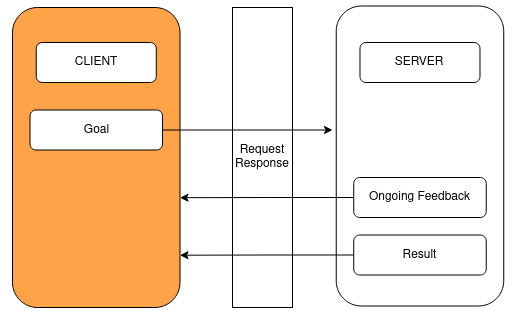
\includegraphics[width=5cm]{images/testbed/microservice/client.png}
%     \caption{The Task Manager Interface includes a State Machine to manage the client.}
% \end{marginfigure}
%\includegraphics[decodearray={0.2 0.5}]{example-image.jpg}

The client requires a decision-maker between each state and a set of possible future states. A state machine is chosen to coordinate the transition between different usecases. For this, the SMACH library is used \cite{smach}. Task handling is implemented with several scheduling elements.

% \begin{marginfigure}%
%   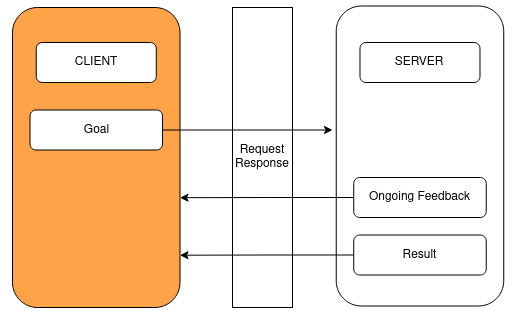
\includegraphics[width=4cm]{images/testbed/microservice/client.png}
%   \caption{An Action \textbf{Concurrence} is executed on the Client side.}
%   \label{fig:taskmanager_concurrence}
% \end{marginfigure}

\begin{itemize}
    \item\textbf{Concurrency}: the ability for a program to be decomposed into parts that can run independently from each other. This means that tasks can be executed out of order and the result would still be the same as if they are executed in order. 
    % An example of a concurrency is listed in Appendix A, Section \ref{code:concurrency}.
    \item\textbf{Preemption}: the act of temporarily interrupting an executing task, with the intention of resuming it at a later time. This interrupt is done by an external scheduler with no assistance or cooperation from the task. 
    % An example of a preemption is listed in Appendix A, Section \ref{code:preemption}.
    \item\textbf{Interruption}: a process tells the task manager to stop running the current program so that a new one can be started. 
    % An example of an interruption is listed in Appendix A, Section \ref{code:interruption}.
\end{itemize}


% \begin{minted}
% [
% frame=lines,
% framesep=2mm,
% baselinestretch=1.2,
% bgcolor=LightGray,
% fontsize=\footnotesize,
% linenos
% ]
% {python}
%     # Part 1: the goal.
%     #
%     # The destination and maximum velocity of the robot
%     geometry_msgs/Point point
%     uint32 max_velocity
%     ---
%     # Part 2: the result, sent by action server upon completion
%     # How many updates thrown in total
%     uint32 updates_n
%     ---
%     # Part 3: the feedback,to be sent periodically by server
%     duration time_elapsed 
                                

% \end{minted}
% %\caption{Example of Action Concurrence Code.}
% \captionof{minted}{\textbf{Template -1:} Example of Action Definition File.}

% ROS consists of a set of executable called nodes, used to perform the system computation. Nodes in ROS are organized in \textbf{Peer-to-Peer} network forming the ROS computation graph.

% Messages transmitted between ROS nodes are simple data structure. They are of two types: topics and services. A topic is a name of a stream of an object published by a node called the publisher. Other nodes interested in this topic may subscribe to it, and they are called listeners. The ROS master node tracks the list of publishers and listeners to a topic. A ROS master node is an XML-RPC server. Nodes connect to other nodes directly. The Master node provides only lookup information, much like a DNS server. ROS uses the transport layer TCPROS for reliably transporting message data. It uses standard TCP/IP sockets.

%%%%%%%%%%%%%%%%%%%%%%%%%%%%%%%%%%%%%%%%%%%%%%%%%%%%%%%%%%%%%%%%%%%%%%%%5

    
\subsubsection{2 | Client-Server Messages}

% \begin{marginfigure}%
%   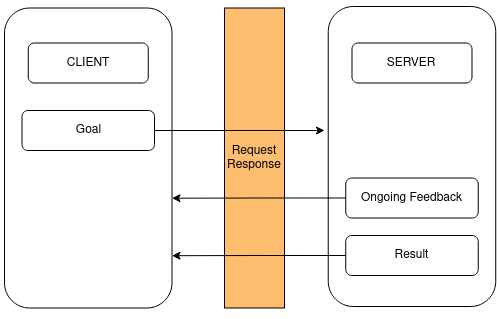
\includegraphics[width=4cm]{images/testbed/microservice/rqrs.png}
%   \caption{Implementation of Message Structure for Request-Response.}
%   \label{fig:marginfig}
% \end{marginfigure}

A message transmits data values during client-server communication. ROS uses a simplified messages description language \cite{ros_docs} for describing the data values (aka messages) that ROS nodes publish. This description makes it easy for ROS tools to automatically generate source code for the message type in several target languages.

\begin{figure*}[!h]
    \raggedright
    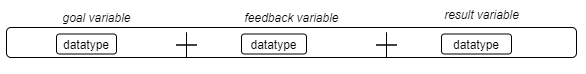
\includegraphics[width=11cm]{images/testbed/microservice/ros_msg_structure.png}
    \caption{Overview of the ROS Message structure.}
\end{figure*}

In an Action Client-Server interaction, communication is ensured ROS Messages with three distinct roles: the goal, the feedback and the result \cite{ros_docs}. An action is executed when the goal requests an action with a set of parameters to the server. Feedback parameters can selected for monitoring during the action's execution. The result informs any concurrent threads of the final state of the action. 


\begin{marginfigure}%[h]
  \raggedright
  \includegraphics[width=5cm]{images/testbed/testbed_arch/one_state_server.png}
  \caption{The client-server interaction.}
  \label{fig:client-server2}
\end{marginfigure}


\subsubsection{3 | Server Handling of Actions}

The Action Server executes an action in the form of a callback functions. A task completes when a particular condition is met. In order to manage this, an action callback can incorporate a condition in its execution. The next section examines this in more depth. 

Each of these pre-loaded behaviours needs to be scheduled. For this, an open-source Function Handler is used, referred to as the ROS Action Server \cite{ros_docs}.As a result, each function for a specific task server will be launched from a central \textbf{launchfile}: 

\begin{figure*}[h]
\raggedright
    \begin{minipage}{1.0\textwidth}
        \begin{minted}
[
frame=lines,
framesep=2mm,
baselinestretch=1.2,
%bgcolor=LightGray,
fontsize=\footnotesize,
linenos
]
{html}
    <launch>
    <group>
        <remap from='_goTo' to='drone1_goTo'/>
        <node name='drone1' pkg='crazyswarm' type='ros_action_server.py'>
        </node>
    </group>
    
    <group>
        <remap from='_goTo' to='drone2_goTo'/>
        <node name='drone2' pkg='crazyswarm' type='ros_action_server.py'>
        </node>
    </group>
    </launch>       
                                        
        
        \end{minted}
        %\caption{Example of Action Concurrence Code.}
        \caption{Example of Server Launchfile with multiple concurrent uses of the same program.}
     \end{minipage}
\end{figure*}

This ROS launchfile loads the functions declared in the Action Server, and remaps them to each drone in the choreography. This allocates a thread under the form of a ROS node. These ROS nodes act as separate Request/Response instances.

\subsubsection{4 | ROS Parameter Handler}\label{parameter_handler} 
The ROS main thread includes a commonly-used component called the Parameter Server, implemented in the form of XMLRPC, and which is, as the name implies, a centralised database within which nodes can store data and, in so doing, share system-wide parameters.


\begin{figure*}[h]
    \raggedright
    \begin{minipage}{1.0\textwidth}
        \begin{minted}
        [
        frame=lines,
        framesep=2mm,
        baselinestretch=1.2,
        %bgcolor=LightGray, 
        fontsize=\footnotesize,
        linenos
        ]
        {python}
        crazyflies:
        - channel: 35
          id: 1
          initialPosition: [0.0, 0.0, 0.0]
          type: default
        - channel: 27
          id: 2
          initialPosition: [1.0, 0.0, 0.0]
          type: default
        - channel: 27
          id: 5
          initialPosition: [4.0, 0.0, 0.0]
          type: default
        \end{minted}
    \caption{Parameter File (.yaml) }
    \end{minipage}

\end{figure*}

Multiple programs query this  file upon initialization of the swarm management layer. Each robot is distinguished by their channel, id and initialPosition. This allows for identifying drone ids and other unique information. 

\begin{marginfigure}%
  \includegraphics[width=5.8cm, center]{images/testbed/testbed_arch/virtual_pin.png}
  \caption{Task Manager interactions with System Architecture}
  \label{fig:taskmanager_pin}
\end{marginfigure}

\subsubsection{5 | Scaling to Multiple Drones}

Similarly to \citename{pradalier_2020}{author}\cite{pradalier_2020}, a procedural task-based programming approach is adopted. This can be likened to a centralized server that services multiple drones. Figure \ref{fig:task_management_architecture} shows the full Task Management Layer Architecture. 

\begin{figure*}[h]
    \raggedright
    \includegraphics[width=11cm]{images/testbed/testbed_arch/task_man_architecture.png}
    \caption{Task Management Layer Architecture.}
    \label{fig:task_management_architecture}
\end{figure*}

This approach values granularity, being lightweight, and the ability to share similar processes across multiple apps. As a result, it is therefore highly reusable for new tasks.


% This condition testing clause is a key element in relating the the server-side monitoring system, to the real execution of the functions. Due to this importance, a simple condition test is displayed here.

% \begin{figure*}[!h]
%     \raggedright
%     \begin{minipage}{1.0\textwidth}
%     \begin{minted}
%     [
%     frame=lines,
%     framesep=2mm,
%     baselinestretch=1.2,
%     bgcolor=LightGray, %#D3D3D3,
%     fontsize=\footnotesize,
%     linenos
%     ]
%     {python}
%     # ACTION EXECUTION EXAMPLE
%     while self.success == False: #While condition is not fulfilled
%         # Conditional check: has drone reached a point?
%         self.success = self._reachedGoal(goal.id, self.initial_pose) 
        
%         ...
    
%     #Once the condition is True: Transition State Machine
%     self.actionServerInstance.set_succeeded() 
%     \end{minted}
%      \caption{Example of Condition Testing. }
%      \end{minipage}
%      \begin{minipage}{0.5\textwidth}
%     \end{minipage}
% \end{figure*}



% \subsubsection{A compatible simulator}
    
% There exists a framework and a simulator that are compatible with this state architecture. Turtlesim provides a simulated 2D turtle (in Fig. X) which is controlled by a ROS topic containing its linear and angular velocity.

% \begin{marginfigure}%
%   \includegraphics[width=4cm]{images/testbed/testbed_arch/turtlesim_bw.png}
%   \caption{Snapshot of the TurtleSim simulator.}
%   \label{fig:turtlesim}
% \end{marginfigure}
\pagebreak
\section{High Level Interface}\label{section:SPI}

% high_level_interface_why}
A high level interface is an abstraction layer for development activities. In order to simplify task development, and align with the thesis goals, we develop a framework for high level interaction between the operator and the functionalities of the testbed.

\subsection{Motivation}

The Testbed, as described in Section. For such purposes, it is required to test user code. Therefore an interface is a key element for the user. There are several advantages to specialised tasks for the testbed.

\begin{itemize}
    \item	\textbf{Handling sub-tasks} to various levels of depth: microservices help automate sub-tasks at a desired complexity. When encapsulated in this way, are separate modules fit for demonstration, that can later be optimised and refined during development.

    \item	\textbf{Monitoring the swarm}: a central monitoring system can run in parallel with the particular algorithms that are tested and validated. For instance, a battery voltage threshold helps to monitor a correct running of the hardware.This allows for preventive maintenance during demonstrations but also during development.
\end{itemize}

In summary, more ‘complex tasks’ will allow for the automation of separate subtasks in a controlled manner.

\subsection{Conceptual Overview}

The high-level interface combines three major elements: 
\begin{itemize}
    \item the management of low-level devices upon each robot,
    \item communication with the swarm, and
    \item scheduling of instructions.
\end{itemize} 

In order to achieve this, the intermediary structures for tasks are laid out here. Figure \ref{fig:loop} labels a hierarchy of tasks. The drone is instructed to alternate between two waypoints until a software condition is triggered.

\begin{figure*}[h]
    \raggedright
    \includegraphics[width=10cm]{images/testbed/SPI/concept_spi_bw.png}
    \caption{Example state machine to implement individual tasks.}
    \label{fig:loop}
\end{figure*}

This example serves to illustrate the conceptualisation of a subtask and a multi-step task. The concurrence of waypoints and the software trigger is consider a sub task, and within a state machine, which is referred to as a multi-step task. This framework offers a definition for complex tasks, as tasks that coordinate the scheduling of instructions, with multi-robot instructions.

\subsection{Architectural Approach}

To create these complex tasks, this high level interface has the following architectural choices:

\begin{itemize}
    \item \textbf{Encapsulating robot instructions } Robot commands are assimilated into this programming interface as individual tasks.
    \item \textbf{Encapsulating swarm instructions } Robot instructions are included in generic functions as swarm instructions.
    \item \textbf{Encapsulating sub tasks} Scheduling processes such as a concurrence runs in a function encapsulating it.
\end{itemize}

This architecture is written in Python, known for its ease of use and flexibility. In this way, multi-step tasks manage the swarm stack, from executing single-robot commands to ensuring the dynamic management of swarms. 

 

\subsubsection{Robot instructions}

\begin{marginfigure}%
  \includegraphics[width=5cm]{images/testbed/SPI/08.png}
  \caption{Example of a robot Instruction.}
  %\label{fig:marginfig}
\end{marginfigure}

The Crazyswarm API from Section \ref{section:swarm} interfaces with low-level hardware for landing, takeoff and further behaviours that can be coded remotely. However, for the purpose of \textbf{centralised task management}, the execution of each instruction should be monitored accordingly. {\citename{hönig_ayanian_2020}{author}} \cite{hönig_ayanian_2020} offer ROS telemetry tools, such as battery monitoring and a reset utility. These can be used as conditions in the execution process. 
Ultimately, an additional layer of abstraction is required for multi-drone instructions. 



\subsubsection{Multi-robot instructions}

\begin{marginfigure}%
    \raggedright
    \includegraphics[width=5cm]{images/testbed/SPI/06.png}
    \caption{Example of a multi-robot instruction.}
\end{marginfigure}%

This section outlines the functions developed \textbf{for group behaviours}: concurrent takeoffs and landings, querying multiple drones for low battery level, etc.  Fly-Octogon and Land-all are examples of multi-robot instructions.

This microservice model is a major component of optimizing swarm programming towards the multipurpose task model outlined in the objectives.

\subsubsection{Sub task management}
\begin{marginfigure}%
    \includegraphics[width=5cm]{images/testbed/SPI/traj_shape_simultaneous.png}
    \caption{Example of a sub task, that includes individual robot instructions, but can also include multi-robot instructions.}\label{diagram:hli_concept}
\end{marginfigure}%

The objective for sub tasks is to assist in creating, and coordinating, \textbf{higher-level behaviours}. An example of this is the concurrent\_traj module, whereas two drones are told to fly simultaneous trajectories. This is of particular interest as two drones will take \textbf{indeterminate amounts of time} to respond to commands. \textbf{Concurrency} — in the context of programming — is the ability for a program to be decomposed into parts that can run independently of each other. 

\subsubsection{Multi-step tasks}

A decision process combines the various modules developed above into a sequence of tasks. This is achieved with a Finite State Machine, which is implemented programmatically with the SMACH python library \cite{smach}. A choreographic state machine is implemented in section \ref{section:choreography}.


\pagebreak
\section{Testbed Demonstration}\label{section:choreography}

A drone choreography is designed as a live demonstration of the Testbed's functionality. The experiment data is accessible publicly \cite{choreography_data}.
 

\subsection{Choreography Design}

 \begin{marginfigure}%
    \includegraphics[width=5cm]{images/testbed/SPI/02.png}
    \caption{Choreography Design: State Machine}\label{diagram:fsm}
\end{marginfigure}%

The State Machine for the full choreography is available in Figure \ref{diagram:fsm}. This demonstration includes:
\begin{itemize}
\item Takeoff and landing, separately and concurrently.
\item A pre-loaded trajectory, from a Bezier curve: concurrently.
\item A polygonial shape flown by two drones, demonstrating simultaneous movement through a set of waypoints.
\item Autonomous state changes.
\end{itemize}

% As part of the testbed for service drones, this work is a compilation of well-known \textbf{swarm behaviors}, which is offered open-source to practitioners of the Crazyswarm Project \footnote{Repository: https://github.com/ThomasCarstens/swarmStack\_flightarena}. This is the first collection of ‘swarm patterns’ known to-date on this swarm framework.
This state machine functions any number of drones: using the swarm building blocks developed in Section \ref{section:SPI}, the dronesexecute trajectories simultaneously; it then moves to certain waypoints indefinitely. In this case a figure of 8 is executed on both drones followed by an octogon. Finally, upon an operator signal, the drones land. The state machine is such that the drones also land if one does not reach its corresponding waypoint in time. %The exact code for this state machine is document in Section \ref{code:collision_sm}.

\subsubsection{1 | Pre-loaded Trajectory}

\begin{marginfigure}%
    \includegraphics[width=5cm]{images/testbed/SPI/traj_shape_simultaneous.png}
    \caption{Simultaneous pre-programmed trajectories.}\label{diagram:simultaneous_trajectories}
\end{marginfigure}%

Two Figures of 8 are flown simultaneously. The figures of 8 are concurrent Bezier shapes, pre-loaded onboard each drone's trajectory follower \cite{crazyswarm_docs}. This is coded using the high level interface as in Fig \ref{code:exec_Fo8}.

\begin{figure*}[!h]
    \raggedright
    \begin{minipage}{1.0\textwidth}
        \begin{minted}
        [
        frame=lines,
        framesep=2mm,
        baselinestretch=1.2,
        fontsize=\footnotesize,
        linenos
        ]
        {python}
        fig8_sm = concurrent_trajs(selected_drones = ids, traj_id = 8)
        StateMachine.add('FIG8_EXECUTE', fig8_sm, 
                        transitions={'succeeded' : 'NEXT_STATE', 
                                     'aborted' : 'land_all', 
                                     'preempted' : 'land_all'}) 
        \end{minted}
        \caption{Integrating a pre-loaded trajectory in the State Machine}
        \label{code:exec_Fo8}
    \end{minipage}
\end{figure*}

The Figure of 8 is assigned an id of 8. Other trajectories are assigned other ids. The concurrent\_trajs function is thus called upon with the required drones and their required ids.

\subsubsection{2 | Multi-point Trajectory.}


\begin{marginfigure}
    \hspace{0.5cm}
    \includegraphics[width=3cm]{images/testbed/SPI/03.png}
    \caption{Multi-drone and multi-point loop.}
    \label{diagram:choreography_trajectories}
\end{marginfigure}

This state loads a custom trajectory on the drone, which is executed, before moving to an indefinite octogonal trajectory. The use of \textbf{waypoint following} is an automation of the motion to specific points. 


\subsubsection{3 | Topic Monitor}

\begin{marginfigure}%
    \includegraphics[width=5cm]{images/testbed/SPI/05.png}
    \caption{Sub task: monitoring an active topic.}
    \label{diagram:monitor_in_trajectory}
\end{marginfigure}

The use of a \textbf{Topic Monitor} is useful to interface with active topics. For instance, at any one moment that a drone gets too close to a particular point, it initiates a landing. The intended behaviour is represented visually alongside.

This is another such subtask that fulfils the initial goal: monitoring the swarm with preventive measures during demonstration as well as training phases. This is performed programmatically with a concurrence between a drone and the /collision topic. 


\subsubsection{4 | Choreography State Machine}

The previous sections are integrated into a State Machine. The configuration of the state machine is displayed in Figure \ref{fig:fsm}. Individual tasks are coloured in green and swarm tasks in orange.


\begin{figure*}[!h]
    \raggedright
    \includegraphics[width=10cm]{images/testbed/SPI/02.png}
    \caption{State Machine Visualisation }
    \label{fig:fsm}
\end{figure*}

Three drones are positioned about the Flight Arena as in Figure \ref{fig:chore_initialisation}.

\subsubsection{5 | Choreography Execution}

\begin{marginfigure}%
  \includegraphics[width=4cm]{images/chore_pictures/octogon/pic.png}
  \caption{View of the Flight Arena during Experiment.}
  \label{fig:chore_initialisation}
\end{marginfigure}
 The state machine is run on a separate thread as in Figure \ref{code:exec_choreography}.

\begin{figure*}[!h]
\raggedright
    \begin{minipage}{1.0\textwidth}
        \begin{minted}
        [
        frame=lines,
        framesep=2mm,
        baselinestretch=1.2,
        fontsize=\footnotesize,
        linenos
        ]
        {python}
        myswarm = swarmInterface(all_ids = [1,3,5])
        sm0 = myswarm.execTrajandOctogon (ids = [1,3], traj_shape = 8)
        myswarm.start_sm_on_thread(sm0)
        \end{minted}
        \caption{Execution of Multi-step tasks}
        \label{code:exec_choreography}
    \end{minipage}
    
\end{figure*}

This invocation of the state machine clearly shows drone ids [1,3,5] as extracted from the Parameter Server, in order to act as the drones 1,2,3. The trajectory shape 8 refers to the Figure of 8.
    
\pagebreak
\subsection{Results}

We proceed with an inspection of the demonstration. The flightpaths of all three drones are plotted together.

\begin{figure*}[h]
    \raggedright
    \includegraphics[width=13cm]{images/choreography/trajectory_choreography2.png}
  \caption{Full Flightpath of all three drones during the Choreography.}
\end{figure*} 

\begin{marginfigure}%
  \vspace{-0.5cm}
  \includegraphics[width=6cm]{images/chore_pictures/octogon/3d2.png}
  \caption{3D Plot of Octogon Figure.}
\end{marginfigure}

Overall, the flightpaths are smooth. The Figures of 8 are traced distinctly, as well as the two octogons. The figure of 8 of drone 3 is discontinuous, and yet there is no apparent effect on the shape. This suggests that the drone moved beyond the area localized by motion capture. When examining the octogons, the top view shows a near perfect superposition: showing small differences in position of less than 2cm. Finally, a line connects the two shapes. This shows that these figures did actually occur in sequence.

\begin{figure*}[!h]
    \raggedright
    \includegraphics[width=5.5cm]{images/chore_pictures/octogon/front2.png}
    \includegraphics[width=5.5cm]{images/chore_pictures/octogon/top2.png}
    \caption{Hover Experiment: Stability Tests on Flight Arena.}
\end{figure*}

Further inspection of the octogons requires a topview and a sideview. The Octogon is traced very clearly. Near the end of the experiment, there is a noticeable wobble in the blue line. This behaviour is due to a low battery level. A notable difference is the wobble in the xz plane, which demonstrates a loss of precision as the drones get closer to the ground. There is a symmetrical behaviour. Further tests can determine what this is attributed to. 

\begin{table*}[h]
  \footnotesize%
  \begin{flushleft}

    \begin{tabular}{lccl}
      \toprule
      Test Description & Value  \\
      \midrule
  Volume of Flight Arena Localized by Motion Capture                     &  \Paste{flight_arena_localized} \\
      Maximum Flight Error Recorded in Hover Test                     &  \Paste{sample_hover_error} \\
      \bottomrule
    \end{tabular}
  \end{flushleft}

  \caption{Key findings in Chapter \ref{c1}.}
  \label{tab:ch1_findings_discussion}
\end{table*}

\pagebreak
\subsection{Discussion}

% \subsubsection{Authors, theories, definitions}

\begin{marginfigure}%[h]
    \vspace{1cm}
    \includegraphics[width=5.5cm]{images/testbed/discussion/rosbuzz_comparison.png}
    \caption{Swarm stack in the Rosbuzz system \cite{buzz_swarm_stack}}
    \label{diagram:swarm_stack}
\end{marginfigure}


In this chapter, a swarm programming approach is developed along similar lines to \cite{pinciroli_lee-brown_beltrame_2015}, the swarm API that was developed for swarms of nanodrones. Both frameworks load a set of functions, they allow the user to select which drones perform a certain task, and group drones according to the task at hand. While Buzz manages membership with a dedicated hash table, our interface makes use of a global parameter handler \cite{buzz_swarm_stack}. Both architecture allows for the development different modules can be developed independently and related dynamically. 

With a high-level interface, this work concerns itself with a swarm-specific language that is not "too top-down" or "too bottom-up". This distinction is seen with increasing swarm sizes, and for creating user tasks more focused on development, or on improving safety and phone interference for demonstrations. 

\begin{marginfigure}%[h]
    \vspace{1cm}
    \hspace{-0.7cm} \includegraphics[width=7cm]{images/testbed/discussion/copilot_structure_bw.jpg}
    \caption{Copilot on the Flying Machine Arena \cite{fma_paper}}
    \label{diagram:copilot}
\end{marginfigure}

 Figure \ref{diagram:swarm_stack} demonstrates that Buzz uses comparable structures for swarm engineering.). ROS communicates with device hardware via MAVROS, a ROS library for compatible Micro Aerial Vehicules. It then has a control distribution layer that is comparable to our Task Manager, a swarm communication layer like Crazyswarm and a swarm control layer like our high level interface. The swarm stack in other research may be composed of other technologies, but retains this structure.

The Flying Machine Arena \cite{fma_paper} is an active area of research for drone development and demonstration, and their 'Copilot' is described as a flight monitoring solution. Figure \ref{diagram:copilot} demonstrates the types of activities achieved via the copilot: updating drone poses during code execution (a), executing playback on recorded poses (b), and executing procedures in simulation (c). These elements are handled by the Task Manager described in this chapter, demonstrating the pertinence of a flight management solution.

% The scheduling of these tasks is a critical difference, as Buzz uses an onboard virtual machine that is very light (12KB), and we opt in this paper for the ROS Parameter Server as a shared parameter space, as well as the ROS Action Server as a shared function space. These are certainly more cumbersome than the distributed data structures of Buzz (sharing data via virtual stigmergy). However, the present architecture allows for different modules can be developed independently and related dynamically. This difference is further expanded upon with the testbed's Middleware Solution (Section \ref{section:middleware} ).

The procedural task-based approach of this chapter is not unique: it figures in \cite{pradalier_2020} who develops a generic pythonic form that need not depend on middleware for task management. All in all, this approach can aid in development, in ways that can be outlined here.
\begin{itemize}
    \item preventing mechanical failure upon software failure.
    \item assist in creating, and coordinating, higher-level behaviours.
    \item monitor the state of every UAV asynchronously.
    \item Assist in troubleshooting with a modular layout.
\end{itemize}

\subsection{Summary}

% testbed_summary
This flight has demonstrated multiple working functionalities. The first is the use of the Swarm Programming Interface. Using the building blocks developed in this chapter, it is possible to develop a multi-stage process, one that includes preloaded trajectories as well as waypoint trajectories, choreographic positioning, and escape cases upon a system abort. With such tools for assistance during development, this set of functionalities pushes beyond previous work, as it offers a layer beyond the crazyswarm's robot instruction set.

\pagebreak
\section{Chapter Summary}


The proposed state-based architecture is a first step towards creating UAV operations to perform complex tasks, collaboratively or otherwise.  After all, this framework has put in place the monitoring tools and the task-based framework to execute complex behaviours; and beyond that, putting in place a Flight Arena has already helped to validated these tools. Such services can easily be tested and deployed from a framework like this one.

Certain elements in this framework are taken a step further in Chapter \ref{c2}: the ability to send streaming setpoints to a drone opens the possibility of flight piloting through other means. This would not be possible without the foundation established in this chapter: the drone architecture, the motion capture setup and the swarm framework.

The tools that were established here may need to be challenged by further research. One direction is the decentralisation of agents with respect to the platform: where this framework has a central role in allocating behaviours, one would opt for a framework that gives each agent the ability to act independently. However, the central monitoring can remain a major asset when developing such a swarm, as it serves as a safety recourse to prevent any hardware damage.

% c1_approach
The testbed makes great use of distributed networking, and it aligns with the first approach of the thesis for task creation. From handling specific parameters, to managing the task execution and scheduling in a centralised manner, the middleware monitors the different agents in an asynchronous manner. As opposed to non-distributed systems, such as direct one-to-one links to onboard devices,  it allows the developer to divert their focus from system communication to performance-critical applications. 
